%!TeX root = main.tex
\documentclass[main.tex]{subfiles}

\begin{document}
	
\chapter{Topology of crystalline materials}\label{topology}
\clearpage



%\documentclass[submission, Chem]{SciPost}

%\newcommand\hmmax{0}
%\newcommand\bmmax{0}
%
%\usepackage{amsmath}
%\usepackage{graphicx, xcolor}
%\usepackage[english]{babel}
%\usepackage{booktabs}
%\usepackage{enumitem}
%
%\usepackage[version=3]{mhchem}
%
%\usepackage{xparse}
%\usepackage{stmaryrd}
%\usepackage{dsfont}
%\usepackage{bm}
%\usepackage{subcaption}
%\usepackage{siunitx}
%
%\frenchspacing
%
%% Shortcuts
%\newcommand{\N}{\mathbb{N}}
%\newcommand{\R}{\mathbb{R}}
%\newcommand{\Q}{\mathbb{Q}}
%\newcommand{\Z}{\mathbb{Z}}
%\newcommand{\eps}{\varepsilon}
%\newcommand{\transp}{{}^t\!}
%\renewcommand{\cal}[1]{\mathcal{#1}}
%
%\newcommand{\OZ}{0_{\Z^3}}
%\newcommand{\OQ}{0_{\Q^3}}
%
%\newenvironment{disj}[1]{\left\{\begin{array}{#1}} {\end{array}\right.}
%\renewcommand{\brack}[1]{\left\llbracket#1\right\rrbracket}
%\newcommand{\der}[2]{#1^{\left(#2\right)}}
%\newcommand{\paren}[1]{\left(#1\right)}
%\newcommand{\abs}[1]{\left|#1\right|}
%\newcommand{\norm}[1]{\left\|#1\right\|}
%\newcommand{\set}[2]{\left\{#1\,\middle|\,#2\right\}}
%\newcommand{\Id}{\text{Id}}
%
%\renewcommand{\t}{\text}
%

%
%% Prevent all line breaks in inline equations.
%\binoppenalty=10000
%\relpenalty=10000
%
%\hypersetup{
%	colorlinks,
%	linkcolor={red!50!black},
%	citecolor={blue!50!black},
%	urlcolor={blue!80!black}
%}
%
%\usepackage[bitstream-charter]{mathdesign}
%\urlstyle{sf}
%
%% Fix \cal and \mathcal characters look (so it's not the same as \mathscr)
%\DeclareSymbolFont{usualmathcal}{OMS}{cmsy}{m}{n}
%\DeclareSymbolFontAlphabet{\mathcal}{usualmathcal}

This chapter introduces the \texttt{CrystalNets.jl} software for crystal topology identification, developed during this PhD. Its content is adapted from \cite{CrystalNets}.

\section{Notion of topology}


\subsection{Definition}

\label{topology_introduction}

In order to describe the average structure of crystalline materials at the nano-scale, reticular chemistry \autocite{reticularChemistry, reticularSynthesis} proposes to classify crystals, and in particular framework materials, in light of their topology. This approach consists in abstractly regrouping the atoms of a crystal into clusters, called \emph{vertices}, bonded together by an abstract kind of linkers, called \emph{edges} --- the choice of grouping being informed by chemical sense. In simple compounds, such as dense oxides, the mapping can be trivial, with each atom as a separate vertex and each chemical bond as an edge. For zeolites and pther aluminosilicates, the tetrahedral atoms T are considered the vertices (T = Al, Si, P, \ldots) and the T--O--T linkages are the edges. In the case of metal--organic frameworks (MOFs), the vertices would be chosen among the \emph{secondary building units} (SBUs) \autocite{SBUs} with more than 2 points of extension, and the edges would correspond to bonds between those as well as ditopic SBUs, for example. Any crystal can then be simplified into a topological structure, called a \emph{net}, consisting of the sets of vertices and edges (see \cref{fig:mof}).

\begin{figure*}[p]
	\centering
	\begin{subfigure}[t]{0.5\linewidth}
		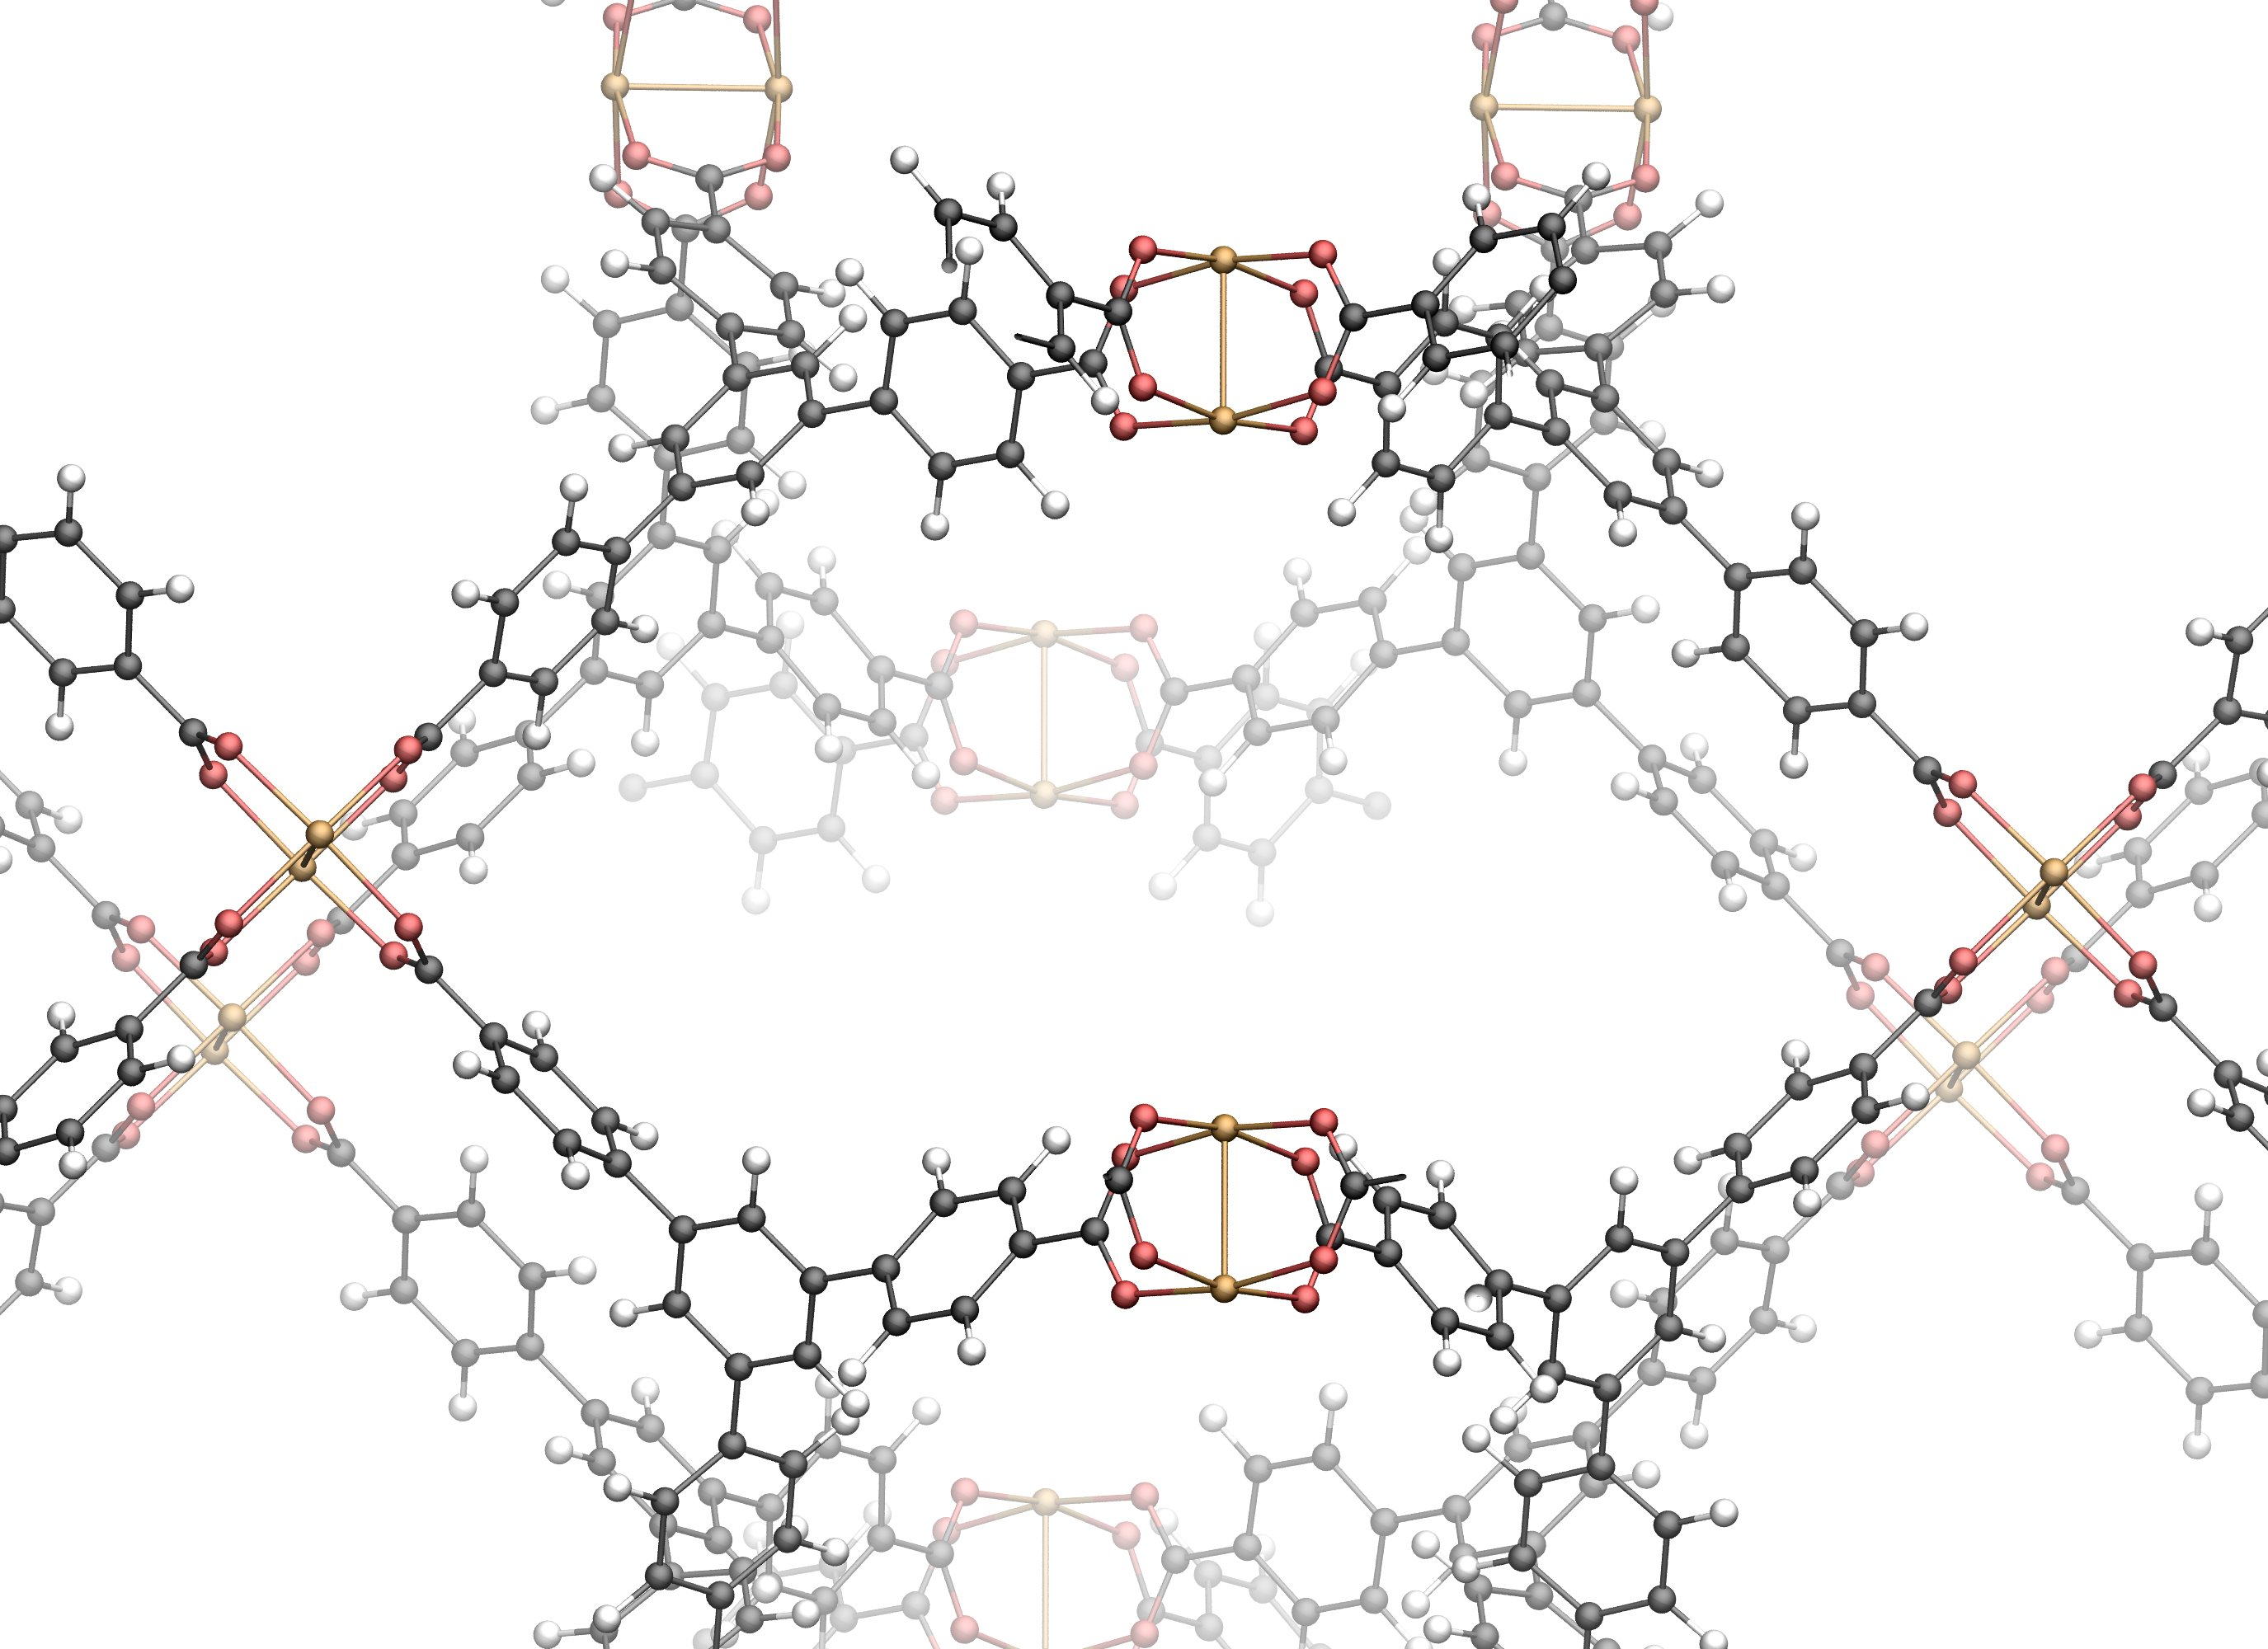
\includegraphics[width=\linewidth]{figures/topology/mof14_1.jpg}
		\subcaption{}
	\end{subfigure}\\[5mm]
	\begin{subfigure}[t]{0.5\linewidth}
		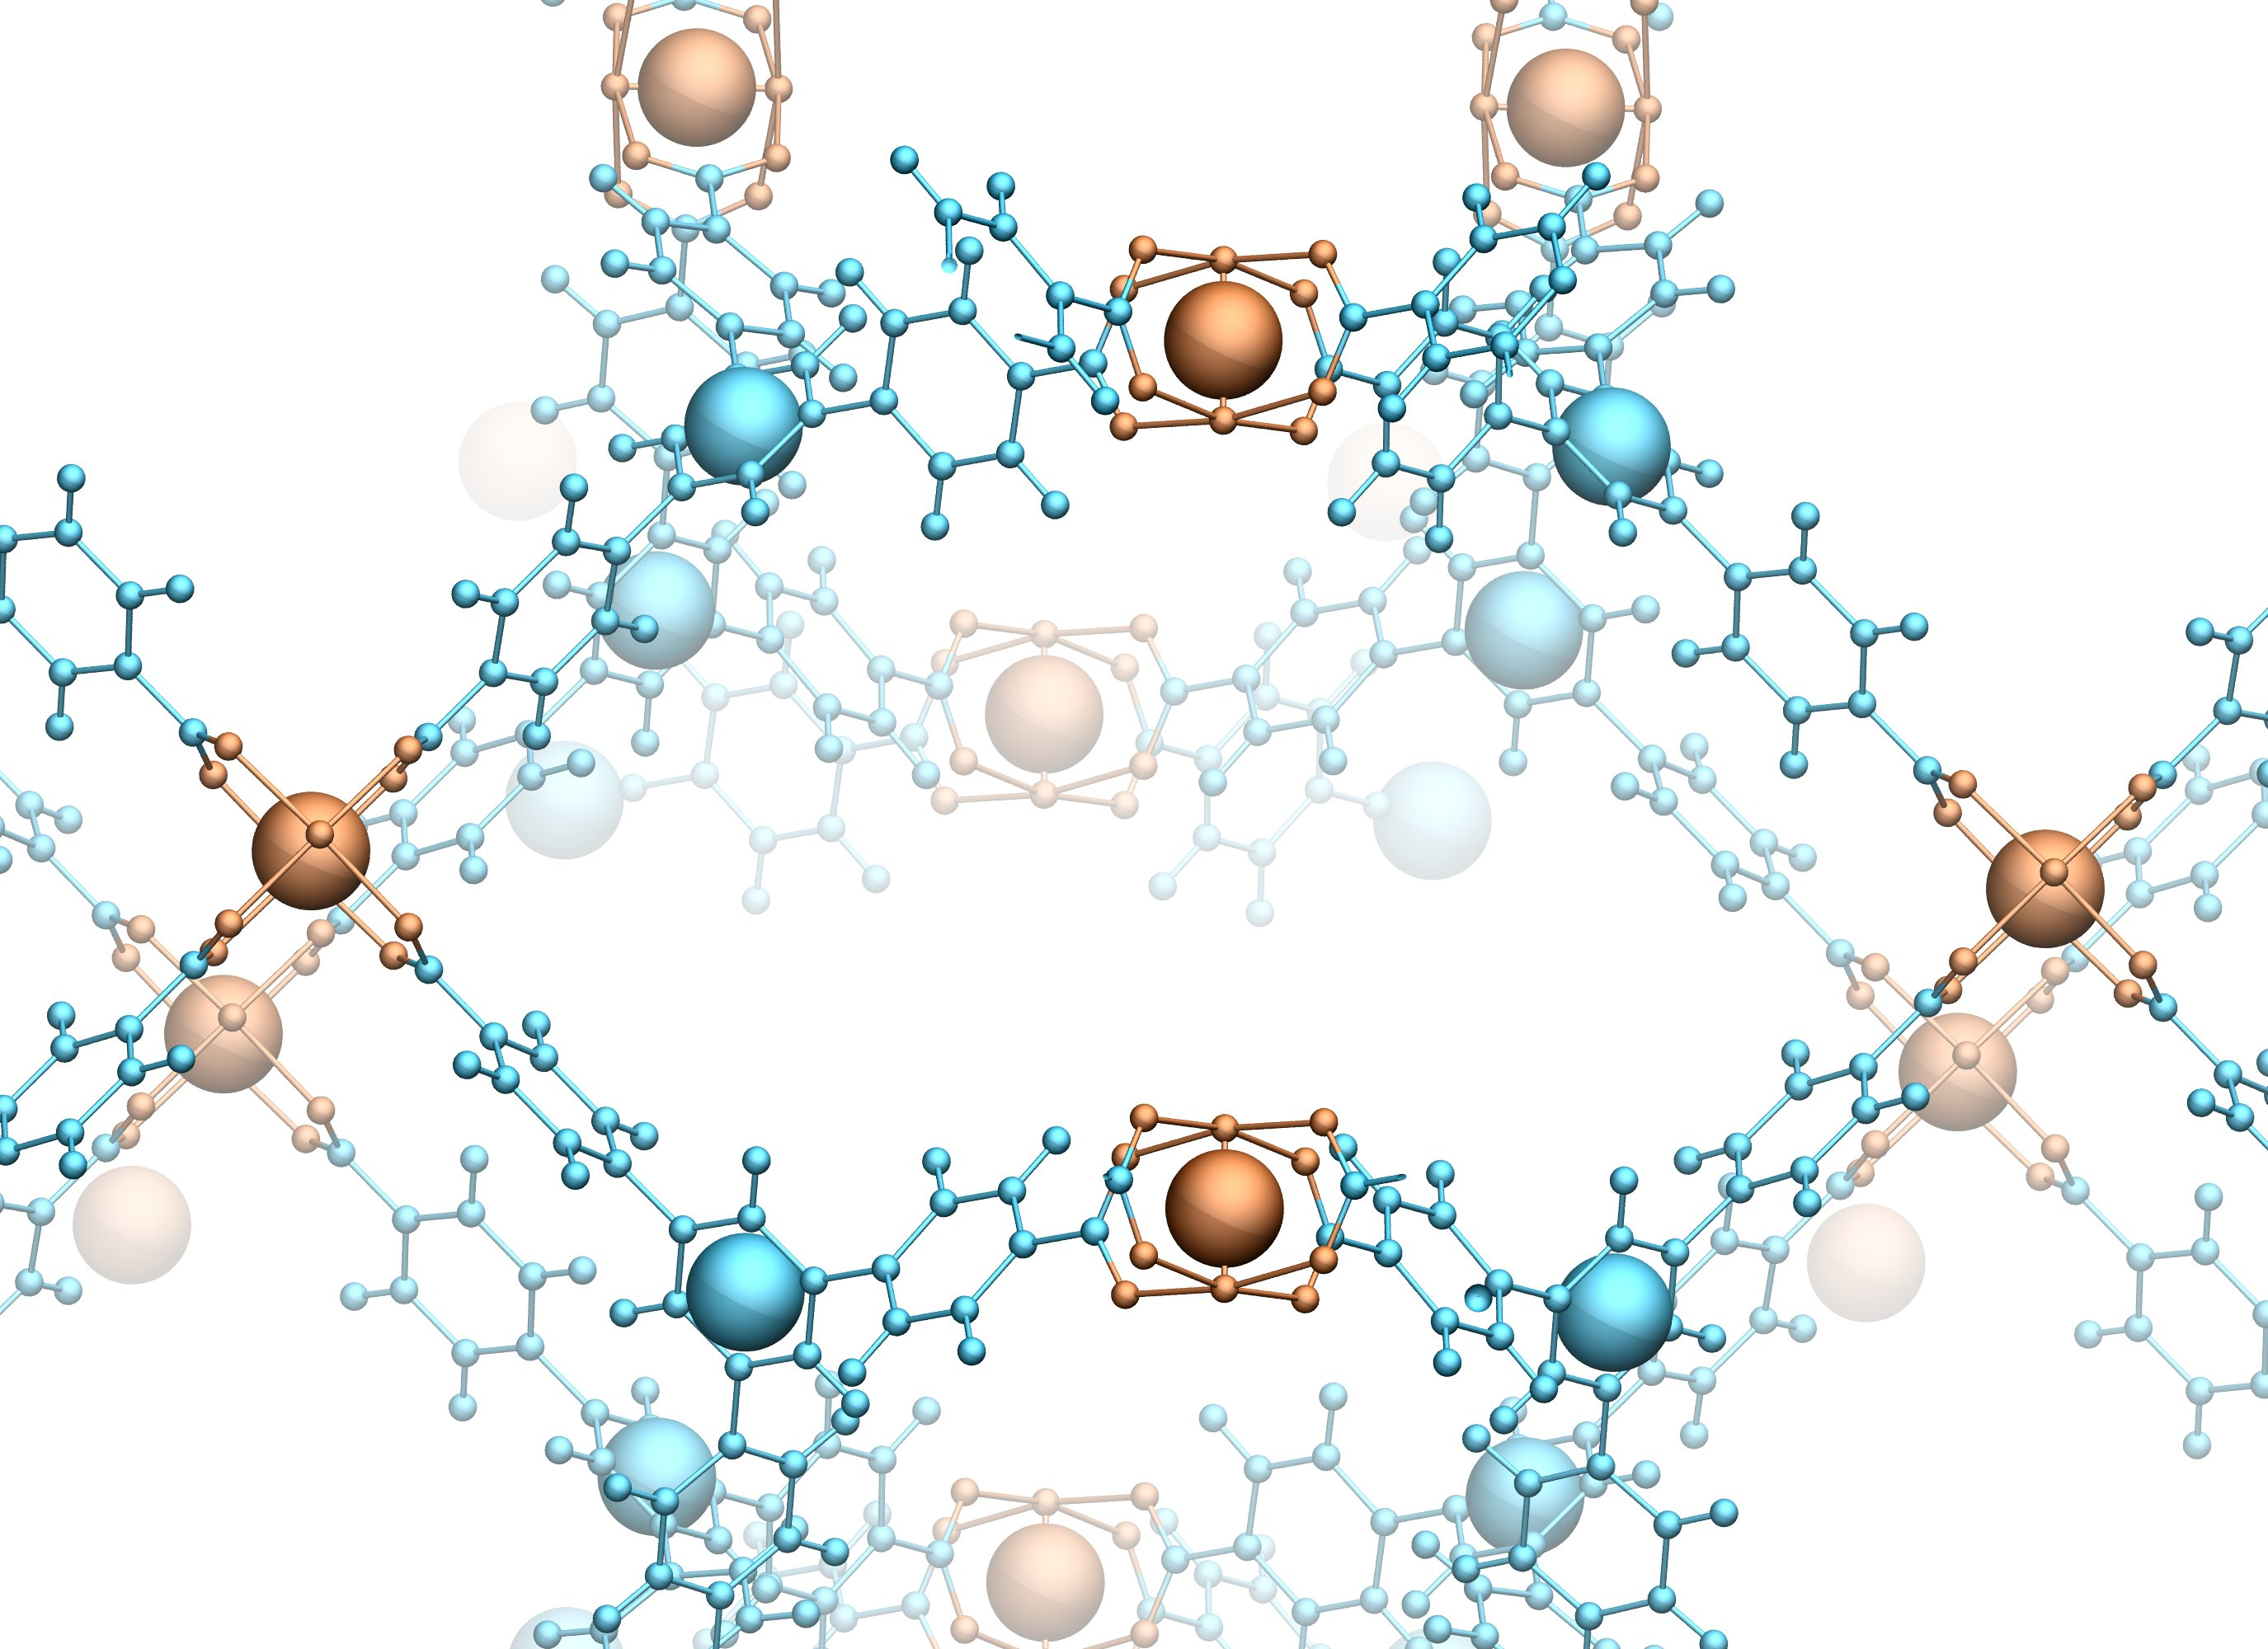
\includegraphics[width=\linewidth]{figures/topology/mof14_2.jpg}
		\subcaption{}
	\end{subfigure}\\[5mm]
	\begin{subfigure}[t]{0.5\linewidth}
		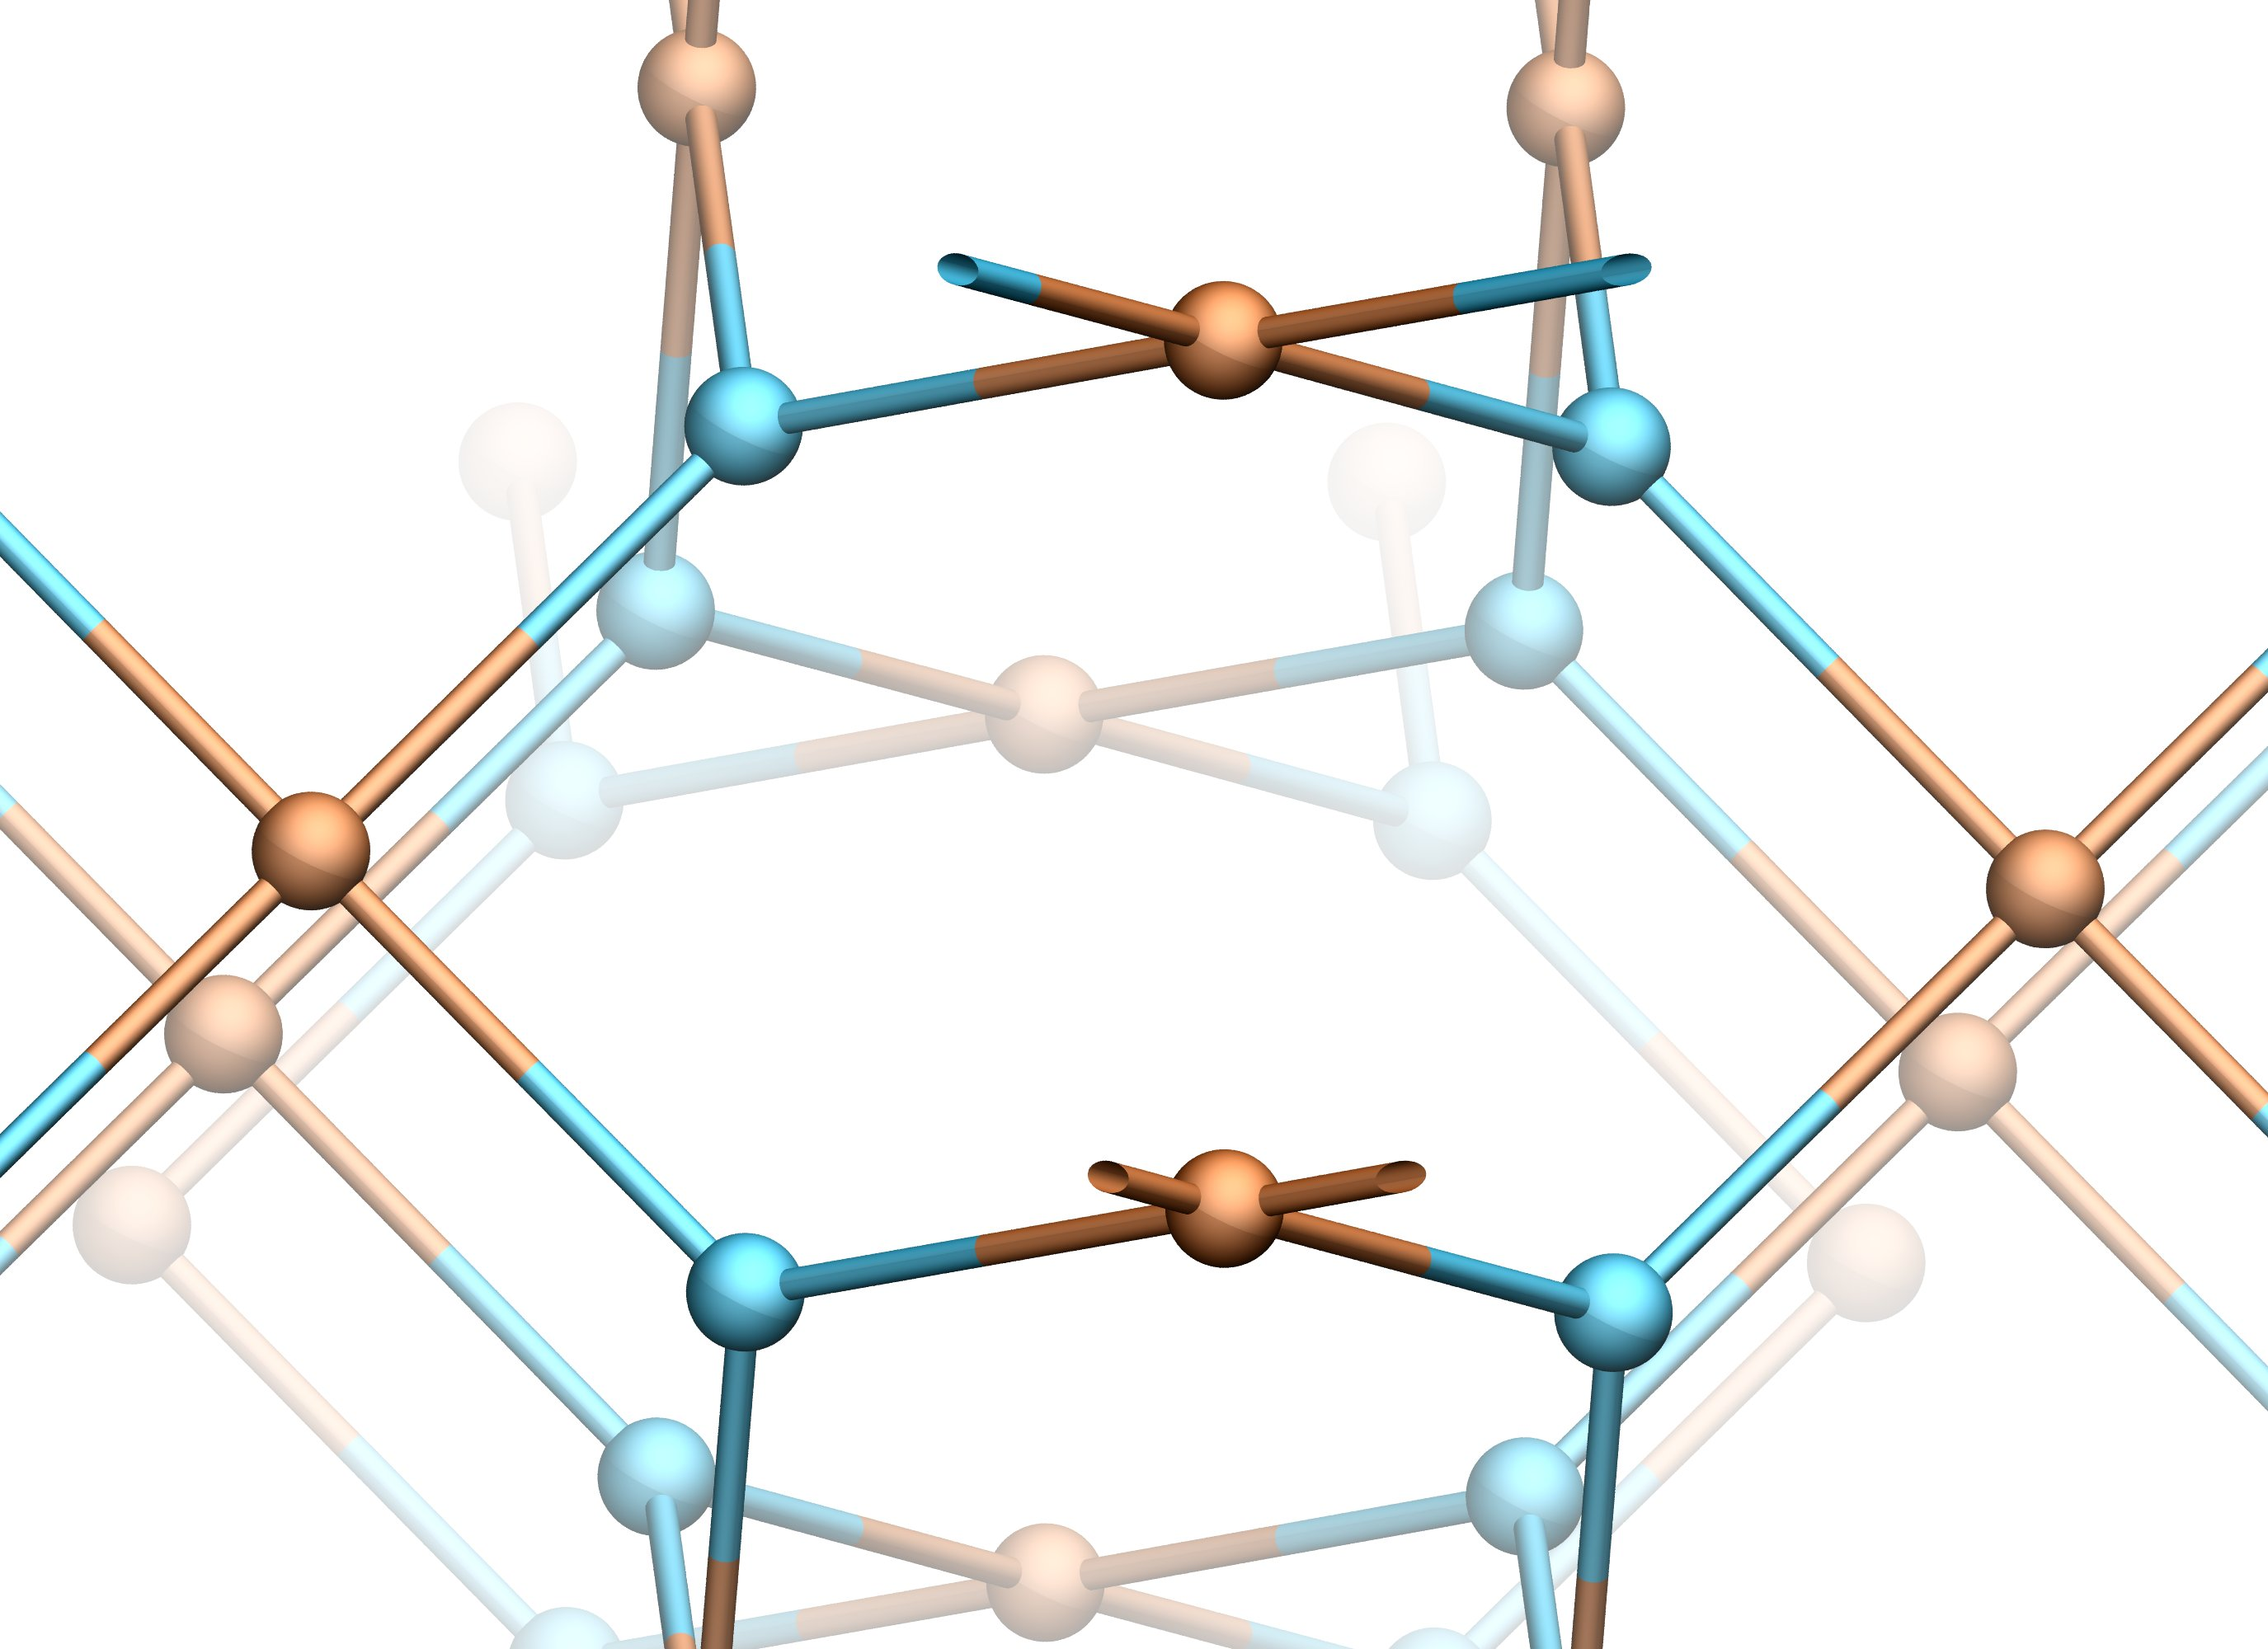
\includegraphics[width=\linewidth]{figures/topology/mof14_3.jpg}
		\subcaption{}
	\end{subfigure}\\[5mm]
	\caption{Decomposition of a crystalline framework into its underlying net:\\
		(a) Crystalline structure of MOF-143 \autocite{MOF143}.\\
		(b) Identification of the SBUs: Cu-based paddle-wheel \autocite{ReverseTopologicalApproach} and benzene-tribenzoate (BTB) \autocite{BTB}.\\
		(c) The underlying net, called \textbf{pto} in the database of the RCSR \autocite{RCSR}.} \label{fig:mof}
\end{figure*}

Like the atomic structure it represents, the net is 3-dimensional and periodic. It contains all the information on the connectivity of the vertices, \textit{i.e.} which pairs of vertices, called \emph{neighbours}, are linked by an edge. Thus, it provides a convenient mathematical abstraction to classify crystal structures. However, it is important to note that this representation is dependent on the choice of vertices and therefore a crystal may be represented by different nets \autocite{OKeeffe}. Moreover, reconstructing the full crystal from the net necessitates additional data, such as the unit cell parameters and the nature and exact geometric placement of the vertices and the edges \autocite{ReverseTopologicalApproach}. A crystal may also be composed of multiple interpenetrating nets \autocite{interpenetration}, which is common in ultraporous framework materials.

\subsection{Existing resources}

Several existing projects, such as the RCSR \autocite{RCSR} or Epinet \autocite{Epinet0,EPINET}, aim at collecting the different nets underlying the structure of real or hypothetical crystals. This is key to allowing researchers to create new materials with a target topology, which is useful to obtain specific physical properties, given the strong link between materials topology and properties for a given chemical composition \autocite{ZIF}. However, in order to check the accuracy of the collected nets with regard to existing crystals, one needs a way to determine the net from a given crystal structure.

There are two different approaches to solve this problem, which correspond to the two main softwares used in the field: ToposPro \autocite{ToposPro,TOPOS} and Systre \autocite{Systre}. ToposPro is a crystallographic tool that allows to retrieve an extensive set of topological properties from crystals. It is a proprietary software, but its topology detection tool can be accessed for free online \autocite{TopCryst}\footnote{available online at \url{https://topcryst.com/}} for crystallographic files in CIF format \autocite{CIF}. Its strategy to identify the topology of a net consists in computing three specific properties for each vertex $u$:
\phantomsection{}
\label{coordinationsequence}
\begin{itemize}
	\item The coordination sequence up to distance 10.
	A vertex $v$ is at distance $k$ of $u$ is there is a chain of $k+1$ vertices $u = u_0,u_1,\ldots,u_k = v$ such that for all $i$ in $\brack{1,k}$ (where $\brack{a,b}$ designates the set of integers between $a$ and $b$), $u_{i-1}$ and $u_i$ are neighbours, and there is no smaller such chain. The $k$-th term of the coordination sequence of $u$ is then defined as the number of vertices at distance $k$ of $u$.
	\item The point symbol.
	\item The vertex symbol.
\end{itemize}
The latter two account for the shortest cycles and rings starting at vertex $u$ \autocite{Definitions, Terminology}.
It is found empirically that the combination of these three properties for all vertices forms an almost unique identifier of the topology. However, this approach is not completely sound as there can be different nets that do share these same three properties.

Systre is an open-source software\footnote{available online at \url{http://gavrog.org/}}; its inputs are files representing the graph underlying the crystal structure, rather than the crystallographic files directly. It implements an algorithm that yields a so-called \emph{topological genome} \autocite{genome} of the net, which is a finite series of numbers. This genome is provably unique for each net, only depends on the net itself and not its representation, and can be computed in polynomial time of the size of the net. To do so, Systre starts by computing an \emph{equilibrium placement} \autocite{barycentric} of the vertices, which attributes to each vertex a position which is the barycentre of that of its neighbours. The net is then minimised, which amounts to finding a unit cell. Afterwards, Systre collects a number of \emph{candidates}, which are frames of reference that do not depend on the current representation of the net. For each candidate, the vertices of the net are ordered according to their position in the frame of reference, and a key is determined which uniquely identifies the net with this ordering in this frame. The genome is then chosen as the lexicographically smallest key. Since the candidates do not depend on the initial representation of the graph, the keys do not either, hence the genome is indeed uniquely determined and only depends on the net itself. In graph theory, the problem Systre solves is called \textit{graph canonization}. It incidentally allows determining whether two input graphs are actually two representations of the same graph (the \textit{graph isomorphism} problem) by comparing their canonical forms (here, the genome), but it can also be used to give a canonical name to graphs for example, by accessing a database of names with the canonical form of the graphs.

Apart from ToposPro and Systre, a few alternative tools have been developed to simplify structures into topological descriptors, but none are suitable for topology identification of chemical structures at large. Indeed, they either only work on specific structures (usually zeolites) like TOTOPOL \autocite{Totopol}, or rely on a non-unique representation of the structure (such as a tiling \autocite{Tiling}) like the T-ring representation \autocite{ChemicalHieroglyphs}, or because their output is not unique for each input structure, like the Single Repeating Unit representation \autocite{GandhiGraphTheoreticRepresentation} for example. For finite molecules, the two most common representations are the SMILES \autocite{SMILES} file format, which is proprietary and comes with several conflicting implementations, or the IUPAC's International Chemical Identifier (InChi) \autocite{InChi} key, which is open-source and more standardized, but less human-readable. Both include additional chemical information as well.

%In this context, my goal is to revisit in detail the algorithm used by Systre in order to improve its usability.
%My work tackle two points:
%\begin{itemize}
%	\item Improve the performance of the software in order to make it able to handle very big nets, such as those underlying the simulation of non-crystalline materials under periodic boundary conditions.
%	\item Add more possibilities of inputs and outputs, so that non-expert crystallographers may find it easy to use with their specific file format.
%	\item In this report, highlight the implementation details of the Systre algorithm.
%\end{itemize}
%I did not work on the existing open-access source code of Systre (written in Python, Java and JavaScript), but instead provide my own reimplementation of the algorithm in Julia \autocite{Julia}, a modern general-purpose and scientific programming language that offers both greater performance and ease of programmability \autocite{JuliaDesign}. This allowed me to improve its performance, which is useful to handle very big nets, such as those underlying the simulation of non-crystalline materials under periodic boundary conditions -- a long-term research goal in the Chimie ParisTech group. In this report, I will revisit the Systre algorithm and highlight the details of my implementation.

\medskip

In this context, I developed a new tool to efficiently determine the topology of crystal structures: the Julia package \texttt{CrystalNets.jl}\footnote{available online at https://github.com/coudertlab/CrystalNets.jl}. Julia \autocite{Julia} is a modern general-purpose and scientific programming language that offers both great performance and ease of programmability \autocite{JuliaDesign}. This, as well as carefully chosen optimisations, allows \texttt{CrystalNets.jl} to outperform Systre while leveraging a very similar core algorithm to ensure soundness. Moreover, the package uses the Julia port of chemfiles\footnote{available online at \url{https://chemfiles.org/}} which allows it to read common chemical file formats like CIF, making it easy to use for the analysis of single cases as well as large databases of crystal structures.

Delgado-Friedrichs and O'Keeffe \autocite{Systre} explained the overall architecture of the Systre algorithm which \texttt{CrystalNets.jl} largely reuses: we will follow its structure, only briefly summarising the key concepts that are already explained elsewhere along the way, while focusing on the implementation choices and some proofs of correctness that do not appear in other publications. We will then focus on a series of new optimisations of the algorithm that allow to greatly improve its performance for most nets. Finally, we will demonstrate the applicability of the method by analysing several existing crystalline databases using \texttt{CrystalNets.jl}.


\section{Algorithms and implementation}

\subsection{From the chemical structure to the net}

\subsubsection{Bonding algorithm}
\label{bondingalgorithm}

Since the topological information is derived from the bond network, using correct bonds is a necessary prerequisite to any topology recognition tool. Yet, identifying bonds in a crystal is not a clear-cut science. %At one extreme, bonds could be attributed according to relatively simple dogma, like in the valence theory of the late 19th century where each oxygen bears exactly two bonds, four around each carbon, etc.
Following the chemical meaning of a bond, the map of electronic density in the system should theoretically be necessary to establish the bond network of the crystal. A bond would then be detected when the density reaches a certain threshold along the interatomic axis, and the nature of the bond (simple, double, triple) can be derived from the overlap of atomic orbitals for instance. However, using this minute vision of the chemical structure, the value of the threshold results from an arbitrary decision.

The fundamental reason why attributing bonds is cannot be made absolute results from the fact that chemical bonds are no more than a useful convention, rather than a measurable observable. Yet, this convention is not without meaning, otherwise any notion built from it, like the topology in case, would lack sense. Therefore, several bond attributing strategies have been devised, none being proven as the ultimate one. %any bonding algorithm needs some flexibility to account for the various situations which may be encountered.
\\

In the case of \texttt{CrystalNets.jl}, whenever the bonds are not explicitly given, the automatic bonding algorithm starts from the heuristic strategy used by Chemfiles and VMD. First, the smallest distance between all pairs of atoms is computed, ``smallest'' being taken among the translated images of each atom across unit cells. Any distance lower than \qty{0.5}{\angstrom} is considered an input error. Otherwise, two atoms are bonded if their distance is below the minimum of two threshold: the first one is proportional to the maximum Van der Waals radius of all atoms in the structure, and the second is proportional to the sum of Van der Waals radii of the two atoms. The Van der Waals radii were taken from the Blue Obelisk's data repository and slightly modified for a few atoms as in Chemfiles.

From this point, the new algorithm departs from that of Chemfiles and VMD by using multiple additional heuristics. First, the two cutoff values mentioned before are controlled by an option that can be tweaked by the user, to remove some spurious bonds or detect some which are just past the threshold. Additionally, if the structure is a MOF or a zeolite (which is set by the user), then the Van der Waals radius of all metallic atoms is multiplied by 1.5, to account for the larger bonds used in the description of inorganic SBUs.

A number of spurious bonds are then removed from the initial guess resulting from these rules. Some common atoms have fixed maximum valence : hydrogen is limited to 1 neighbour, carbon and nitrogen to a maximum of 4, oxygen to 2 unless it has metallic neighbours, in which case it can have up to 4 neighbours (a typical use case is for metal-oxo clusters). Bonds shorter than \qty{0.65}{\angstrom} or longer than \qty{4}{\angstrom} are removed, as well as those longer than \qty{3}{\angstrom} that are significantly out-of-plane with respect to other bonds around any of the two neighbours. Metal-metal bonds are conditionally removed according to user options. Finally, in a configuration where three atoms are pairwise bonded in a triangle, the longest of the three bonds is removed if it is either too long or too close to the opposite atom.

All these heuristics were derived from manual inspection of the result of the bonding algorithm over databases of crystal structures. As with any strategy relying on heuristics, it cannot be made perfect, but it appears to be reasonable enough for all cases encountered so far. Overall, this strategy works well with respect to the time vs precision trade-off required by \texttt{CrystalNets.jl} ; any input without explicit bond which requires this algorithm will still result in a warning though, to let the user know that the automatically extracted bond network should be carefully checked.

It should be mentioned that some bonding strategies are out of scope of this algorithm, such as the detection of hydrogen bonds, typically. Studying the topology resulting from such a bond network thus requires passing explicit bonds in the input file.



\subsubsection{Clustering algorithms}
\label{clusteringalgorithms}

Once the bond network is obtained, it undergoes clustering, which consists in grouping together sets of atoms: each such cluster will then be collapsed into a single vertex in the net. This transformation is useful in order to simplify the exact atomistic topology into a higher-level topology that can expose the overall organisation of the crystal, without reproducing the low-level details. %For example, any cycle of atoms present in the net will count as a cycle for the low-level topology; however, abstracting this cycle into a single vertex representing the cycle allows significantly simplifying the topology.

\begin{figure}
	\centering
	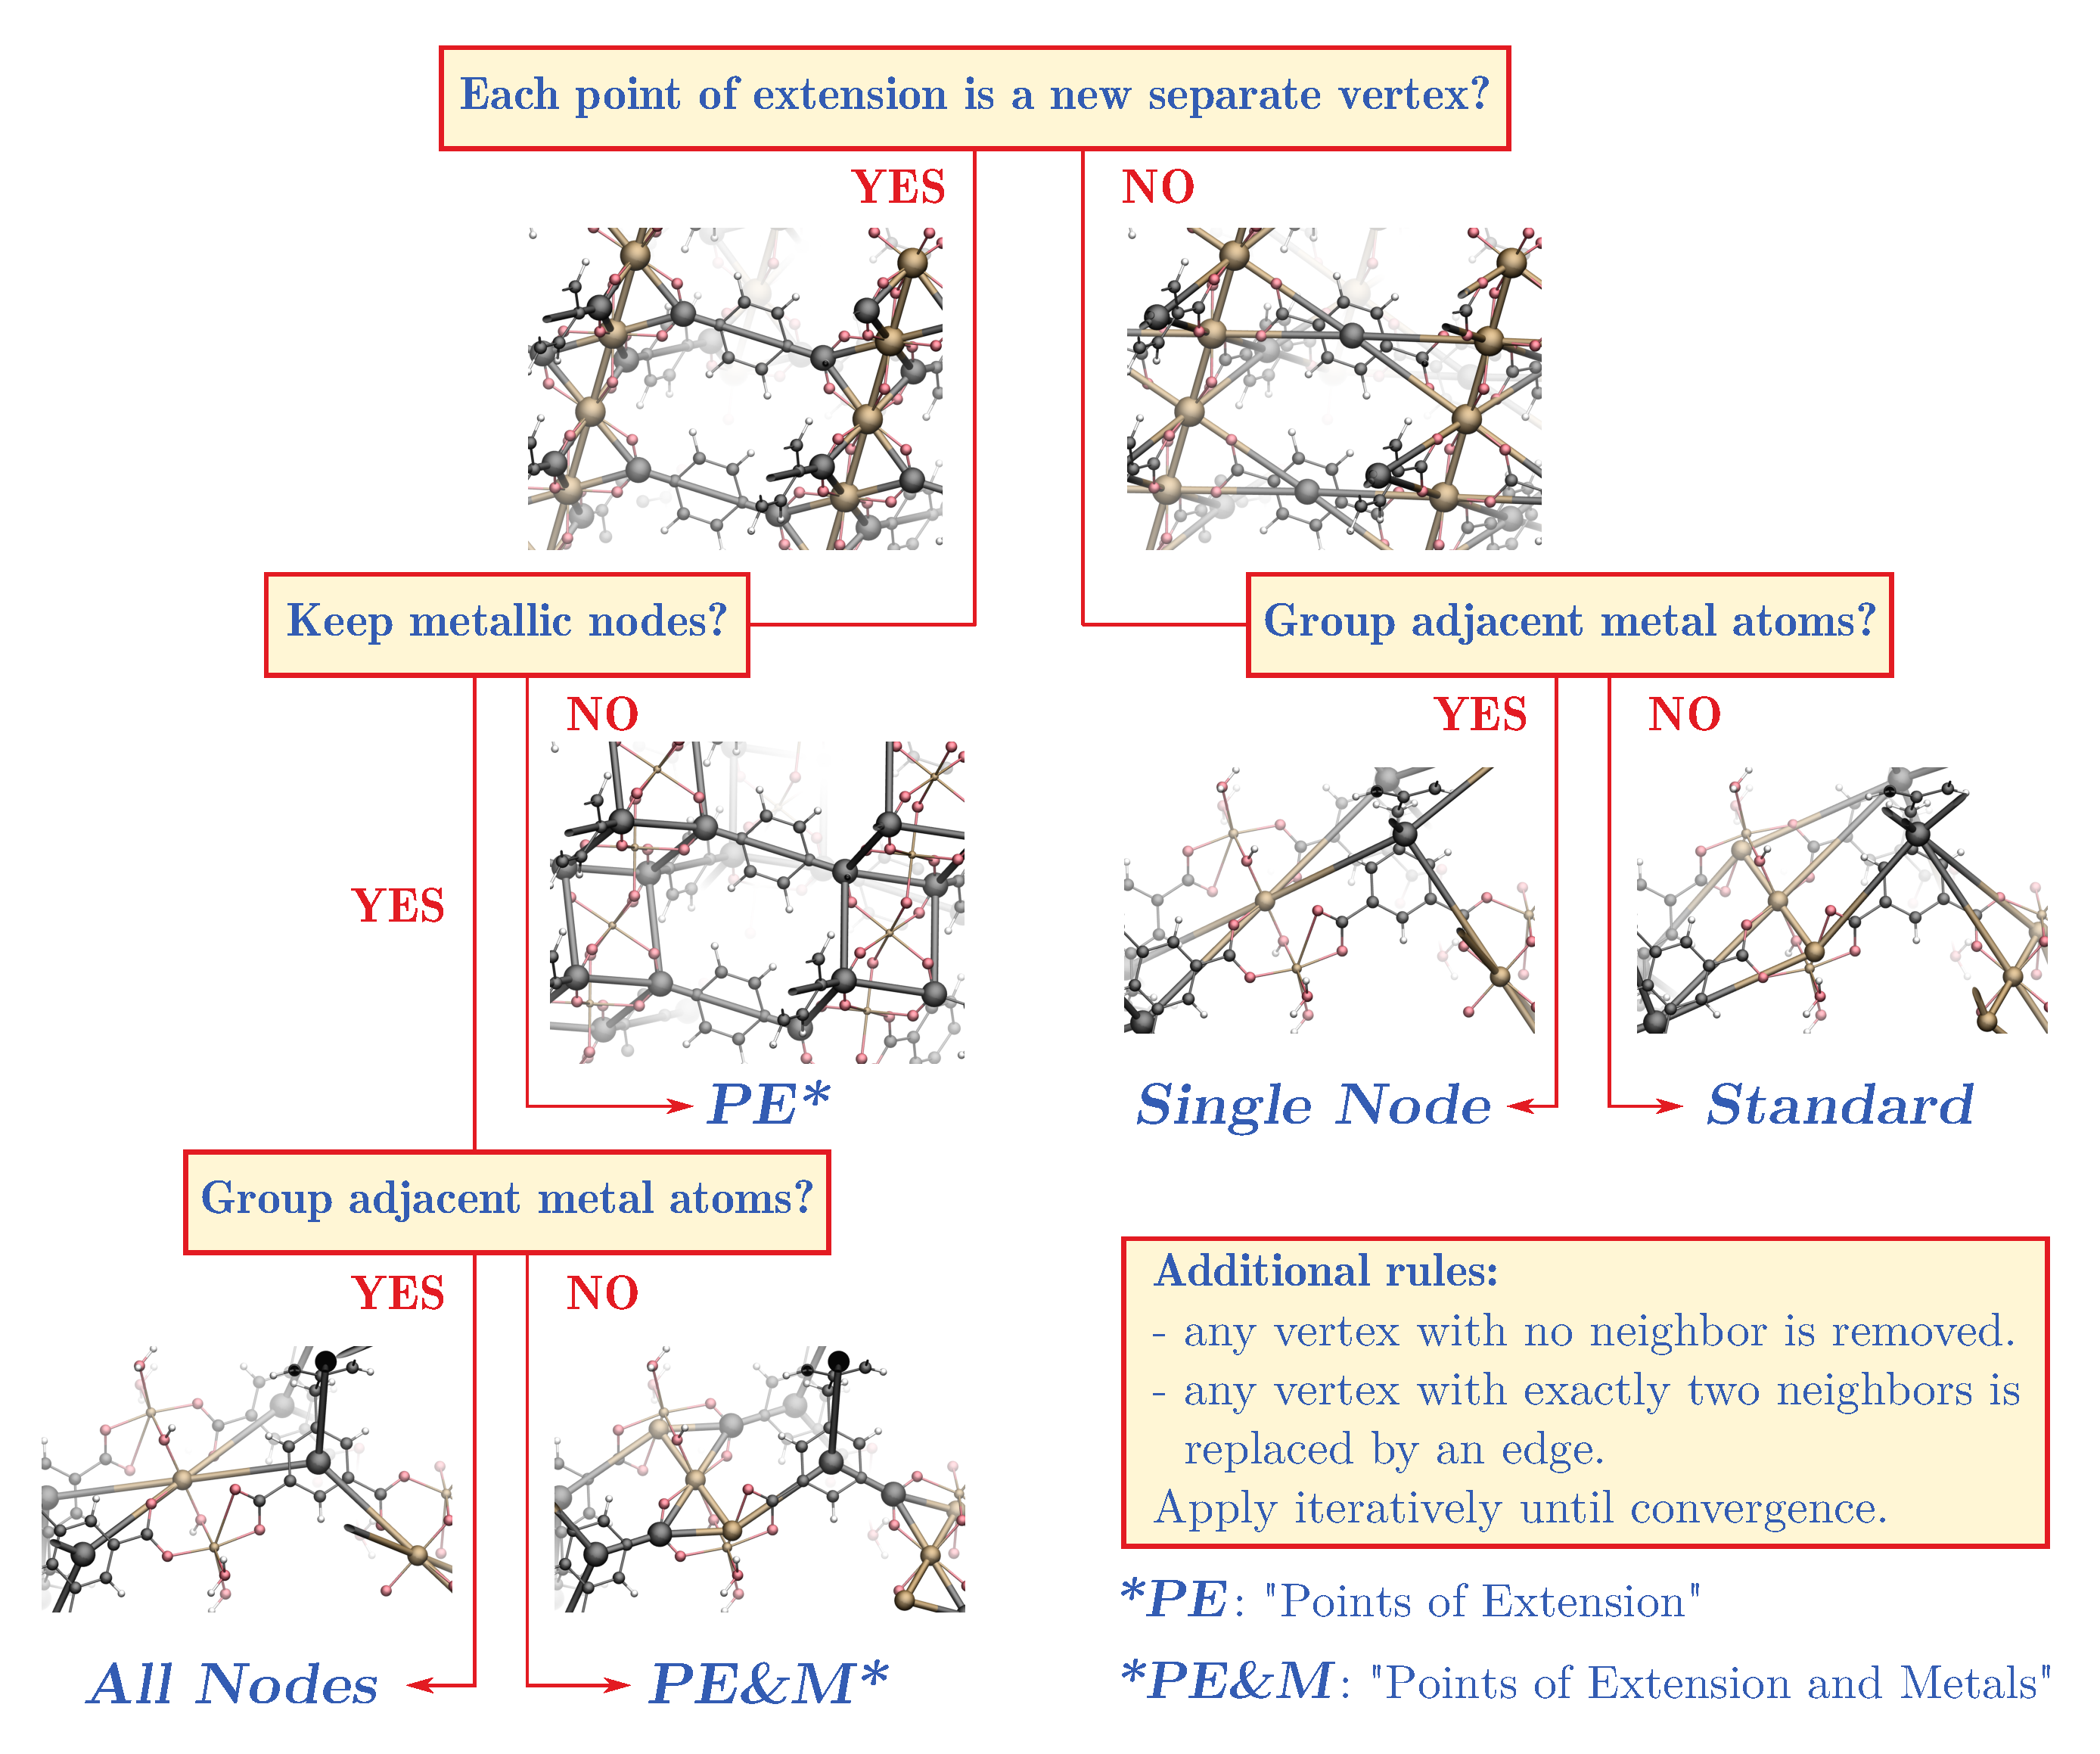
\includegraphics[width=\linewidth]{figures/topology/clustering.pdf}

	\caption{Schematic representation of the key differences between clustering choices}\label{fig:clustering}
\end{figure}

I implemented five main clustering options: ``all nodes'', ``single node'', ``standard'', ``PE'' and ``PEM''. All decompositions start by separating metals, on the one hand, and organic carbons, on the other hand. Aromatic cycles are merged into a single pseudo-atom. The ``Single Node'' strategy\autocite{IUPAC_SBU} consists in growing the metallic clusters, then the organic clusters, with adjacent non-attributed atoms until all have an attributed group. The ``All Nodes'' clustering\autocite{IUPAC_SBU} additionally puts the points-of-extension\autocite{UnifiedTopology,YaghiRodMOFs}, which are the organic atoms bonded to an inorganic cluster, into their own separate group. Alternatively, each metal atom can be put into its own separate group, yielding the ``Standard'' strategy. These three methods have been standardized by IUPAC\autocite{IUPAC_SBU}.

In addition to these three main options, the ``Points-of-Extension and Metals'' (PE\&M) algorithm proposed by \textcite{ProserpioPEM} consists in retaining the points-of-extension from the initial clustering, but discarding those clusters to only keep one per metal atom and one per point-of-extension. Finally, the ``Points-of-Extension'' (PE) strategy only retains one cluster per point-of-extension. All of these differences are summarized in \cref{fig:clustering}.


Except for the ``standard'' representation which is uniquely defined by its implementation in ToposPro \autocite{BlatovSimplify,BlatovCSD}, the other clustering options are only described, like before, but not uniquely determined by an explicit algorithm \autocite{IUPAC_SBU,OKeeffeSBU,OKeeffe,BlatovSimplify,MetalOxo,ProserpioPEM}. \texttt{CrystalNets.jl} does not follow the original implementation of the ``standard'' representation\autocite{BlatovCSD}, primarily because of the required computational cost for determining the minimal ring around each bond. Instead, its custom algorithm consists in the following main steps:
\begin{itemize}
	\item First, organic cycles are replaced by a new virtual carbon atom. Afterwards, all metallic atoms are assigned to the ``inorganic'' class and all carbon atoms to the ``organic'' class. Then, in a loop, each remaining atom that is bonded to an atom in the ``inorganic'' class is itself classified as ``inorganic'', until no such atom remains. All remaining unassigned atoms are then classified as ``organic''. P and S atoms are treated differently and considered organic if directly bonded to a carbon, metallic if directly bonded to a metal, and part of a third class otherwise.
	
	\item Afterwards, SBUs are formed by regrouping together all adjacent atoms belonging to the same class. Paddle-wheel patterns are identified separately and regrouped into a single inorganic SBU even when the two opposite metal centres are not bonded together. The \textit{points of extension}, which are organic atoms bonded to an inorganic atom, form their own SBU each. The algorithm stops here if there is no periodic SBU, \textit{i.e.} if there is no infinite set of adjacent atoms belonging to the same class.
	
	Otherwise, if there are such periodic SBUs, they are split by virtually removing the atoms with the highest connectivity and regrouping the other atoms of the periodic SBU into the remaining connected components. A few other heuristics are used to ensure that all final SBUs are finite, and to tackle the various possible configurations encountered in framework structures.
\end{itemize}

This algorithm yields the ``all nodes'' representation . It can be converted to ``PE'' (standing for ``points of extension'') by removing all metallic atoms and bonding their corresponding points of extension to describe the coordination polyhedra around the removed metals. The ``all nodes'' representation is also convertible to ``single nodes'' simply by merging the organic points of extension with their neighbouring organic SBU. It can also be transformed to yield the ``PEM'' representation by splitting inorganic clusters to keep only one metal atom per SBU. Combining the algorithm for ``PEM'' and ``single nodes'' yields the ``standard'' representation \autocite{BlatovSimplify}. For simple cases, \texttt{CrystalNets.jl} also provides an ``each vertex'' clustering option which bypasses the entire clustering step and keeps each atom as its own vertex in the net, as well as an ``input'' option which determines clusters directly from the \texttt{Residues} of the chemfiles-parsed input file, so that the user may provide their own SBUs.


%All of these clustering options are internally converted to finer-grain options which can be individually toggled on or off. This can allow users to retrieve nets with unusual configurations, for instance without clustering organic cycles into a new vertex, or by keeping edges between two metallic SBUs even in the ``standard'' representation.

Once the SBUs are determined, they are converted to vertices and bonded together according to the atomic bonds. % If one of those vertices is made only of oxygen atoms (usually a single oxygen with three or more atomic bonds [INSERT EXAMPLE?]), then it is removed and all its neighbours are bonded together instead.
Finally, as with all nets in \texttt{CrystalNets.jl}, if a vertex has one or zero neighbour, it is removed, and if it has exactly two neighbours it is converted into an edge between its neighbours, and this iteratively until convergence. Once vertices and edges are defined, interpenetrating nets are separated, each of them accounting for a single structure.\\

Overall, the net which will be identified by \texttt{CrystalNets.jl} heavily depends on a series of choices made when deciding on the bond attribution, as well as the clustering step. Automated tools can only guess so far as to the expected decomposition of the crystal, hence the importance of checking the alignment of the detected net with the expected outcome.


\subsection{Periodic graph structure}

\label{periodicgraphs}

%Conceptually, a crystal can be thought of as a combination of a lattice and a pattern, the latter being repeated on each point of the former. From a computational standpoint, this can be translated into several representations. There is a large variety of crystallographic file formats used to this end but most of them express the same information, which is the geometry of a unit cell and the position of each atom within that unit cell, possibly alongside some information about the symmetries of the crystal, the chemical bonds, the diffraction pattern, etc.

%Another approach, which is the one used by Delgado-Friedrichs and O'Keeffe \autocite{Systre}, disregards the given positions of the atoms and focuses on the graph structure of the crystal.

Crystal nets are special instances of 3-periodic graphs. In general, a \emph{graph} is a mathematical construct that contains objects, called \emph{vertices}, some of which are linked together by \emph{edges}. Two linked vertices are said to be \emph{neighbours}. In a crystal, the pattern representing the atoms and their chemical bonds periodically repeats itself across three dimensions: for this reason, the graph representing a crystal is called 3-periodic.

More generally an $N$-periodic graph (with $N\in\N^*$) can be represented using the vector model \autocite{Chung}. This model conceptually follows the description of a crystal as a lattice and a pattern. Any point in the lattice is denoted by an offset $o\in\Z^N$, whose $i$-th coordinate is the offset along the $i$-th axis of the lattice compared to a fixed origin. An $N$-periodic graph is then defined by a pair $(V,E)$ where $V$ is the set of vertex identifiers and $E\subset V\times V\times \Z^N$ is the set of edges. Any vertex in space is uniquely identified by a pair $(v,o)\in V\times\Z^N$ where $v\in V$ is its vertex identifier and $o\in\Z^N$ is the offset of the cell that contains the vertex. Let's note $n = \left|V\right|$ the number of vertices per cell and identify $V$ with the integer interval $\brack{1,n}$ so that each vertex identifier can be considered to be a number in $\brack{1,n}$. When working in a fixed cell, the vertices will simply be referred to by their vertex identifier.
%For a crystal, the vertex identifiers are additionally labelled with the name of the atom (or cluster of atoms) they represent.
Finally, for most of the rest of this chapter $N$ will be equal to $3$ since nets are 3-dimensional, but the algorithms exposed in the rest of this section actually work for any dimension and \texttt{CrystalNets.jl} can identify 2-periodic and 1-periodic graphs as well.

An edge $e = (u,v,o)$ can be broken down into a source $u\in V$, and a destination $(v,o)\in V\times\Z^3$. The source can be seen as the vertex of identifier $u$ and positioned in the cell at the origin of the lattice, and the destination is the vertex to which it is linked. When the source and the destination are in the same cell, the offset $o$ is zero and noted $\OZ = (0,0,0)$. Edges of the form $(u,u,\OZ)$, called \emph{loops}, are absent in nets because they do not convey any structural information.

For any edge $e = (u,v,o)\in E$, the reverse edge $(v,u,-o)$ is also in $E$: this property makes the graph \emph{undirected}. All graphs used to represent crystals are undirected because chemical bonds are symmetric: if atom $A$ is bonded to atom $B$, then atom $B$ is bonded to atom $A$, and likewise for clusters of atoms.% Beware that the graph being undirected is not linked to its possible symmetries, and in particular $(u,v,o)\in E$ does not imply $(u,v,-o)\in E$.

\medskip

As opposed to periodic graphs, \emph{simple} graphs do not have a concept of offset: an edge of a simple graph is only a pair of vertices. Numerous computational representations of simple graphs exist in the literature, but they cannot be directly transposed to periodic graphs. In order to find a computational representation for crystals relevant to topological analyses, a useful observation is that nets share two distinctive features that come from chemistry:
\begin{itemize}[noitemsep]
	\item The number of edges is at most proportional to the number of vertices, because of the limited valence of atoms. Such graphs are generally called \emph{sparse}. This remains true when vertices represent clusters instead of single atoms, although in that case the number of neighbours can be higher than the maximum valence of an atom --- for instance, SBUs with up to 66 points of extension have been built. \autocite{SBUs}.
	\item The set of edges is small to medium-sized because the number of vertices per unit cell is, in practice, between 1 and 10,000 in most real-world crystalline structures. This is small compared to the trillion of edges of some graphs in social media modelling for instance \autocite{facebook}.
\end{itemize}

Finally, the most important operation on graphs that will subsequently be used is finding the set of neighbours of a given vertex. Driven by this, I chose to computationally represent a periodic graph by a list of size $n$ whose $u$-th element is the set of neighbours of $u$: \linebreak$N_u= \set{(v,o)\in V\times\Z^3}{(u,v,o)\in E}$. $N_u$ is stored as a lexicographically sorted list. %Let's also use $N_{u,o'} = \set{(v,o+o')\in V\times\Z^3}{(u,v,o)\in E}$ to denote the set of neighbours of the representative of vertex $u$ in the unit cell $o'$.

Because of the previously mentioned undirectedness of the graph, if $(v,o)\in N_u$, then $(u,-o)\in N_v$. However, it is often convenient to be able to enumerate the edges of the graph without double counting an edge and its reverse. For this reason, the representation comprises another list of size $n$ whose $u$-th element is the first index $i$ in $N_u$ such that $N_u[i] = (v,o)$ with either $v>u$ or $\big[ v = u\text{ and }o > \OZ \big]$. Such an edge $(u,v,o)$ will be called a \emph{direct} edge. Since loops are forbidden, all edges are either a direct edge, or the reverse of a direct edge. Thus, since each list of neighbours is lexicographically ordered, reading the list of neighbours starting at the given indices $i$ is guaranteed to yield all direct edges of the graph, hence each edge exactly once without its reverse. The lexicographically ordered sequence of direct edges is a unique identifier of a representation $(V,E)$ of a periodic graph in the vector model: such a sequence will be called the \emph{key} associated with the representation.

\begin{figure*}[t]
	\begin{subfigure}[b]{0.35\linewidth}
		\hspace{-1.5em}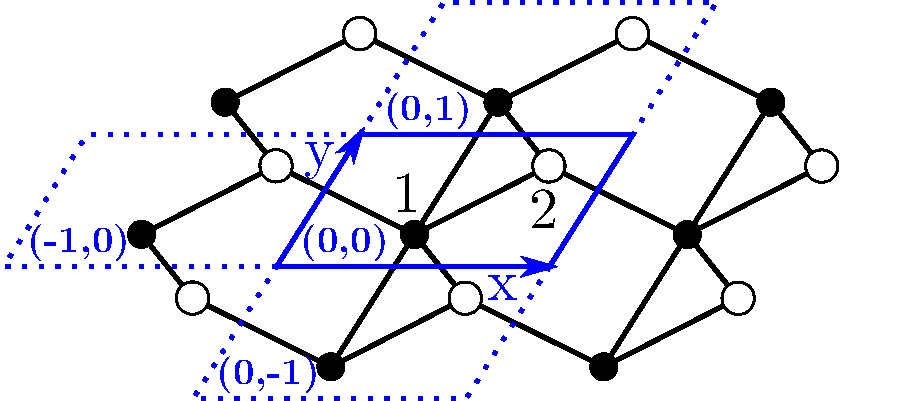
\includegraphics[width=0.96\linewidth]{figures/topology/cells_ref.pdf}
		\subcaption{Reference unit cell}
		
		\centering\begin{tabular}{ccccc}
			1&1&&0&1\\
			1&2&&-1&0\\
			1&2&&0&-1\\
			1&2&&0&0
		\end{tabular}
		
	\end{subfigure}%
	\begin{subfigure}[b]{0.35\linewidth}
		\hspace{-1.5em}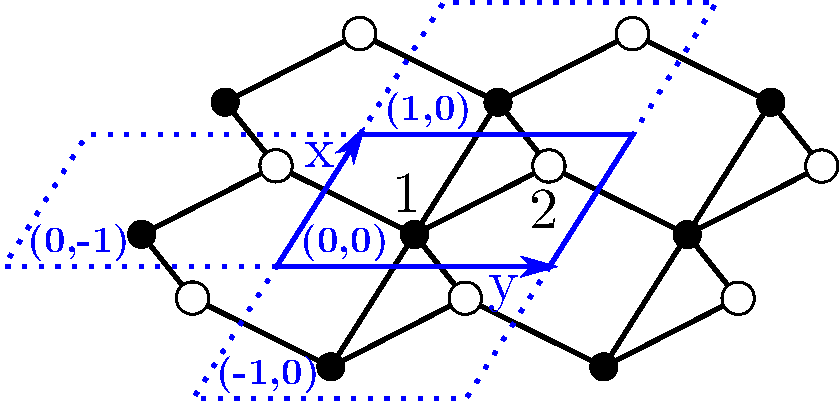
\includegraphics[width=0.9\linewidth]{figures/topology/cells_xy.pdf}
		\subcaption{Inversion of axes}
		
		\centering\begin{tabular}{ccccc}
			1&1&&1&0\\
			1&2&&-1&0\\
			1&2&&0&-1\\
			1&2&&0&0
		\end{tabular}
		
	\end{subfigure}%
	\begin{subfigure}[b]{0.35\linewidth}
		\hspace{-2em}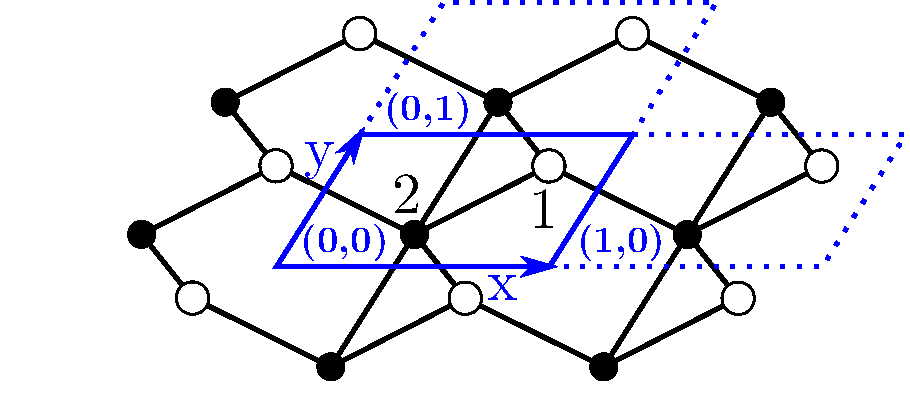
\includegraphics[width=1\linewidth]{figures/topology/cells_12.pdf}
		\subcaption{Renumbering of vertices}
		
		\centering\begin{tabular}{ccccc}
			1&2&&0&0\\
			1&2&&0&1\\
			1&2&&1&0\\
			2&2&&0&1
		\end{tabular}
		
	\end{subfigure}
	\begin{subfigure}[b]{0.35\linewidth}
		\hspace{1.5em}
		\hspace{-2em}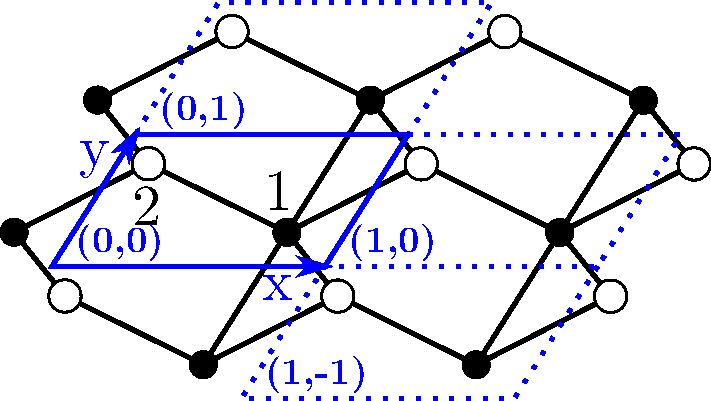
\includegraphics[width=0.8\linewidth]{figures/topology/cells_orig.pdf}
		\vspace{1em}
		\subcaption{Change of origin}
		
		\centering\begin{tabular}{ccccc}
			1&1&&0&1\\
			1&2&&0&0\\
			1&2&&1&-1\\
			1&2&&1&0
		\end{tabular}
		\vspace{-0.5em}
	\end{subfigure}%
	\begin{subfigure}[b]{0.35\linewidth}
		\hspace{-2em}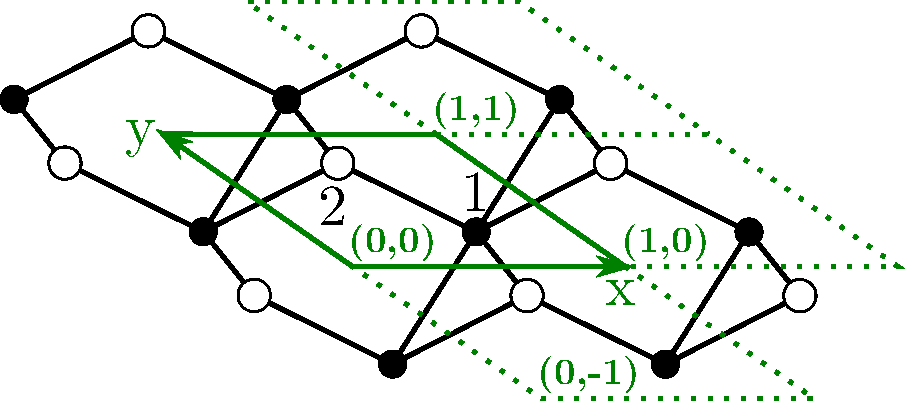
\includegraphics[width=1\linewidth]{figures/topology/cells_other.pdf}
		\vspace{1em}
		\subcaption{Other unit cell}
		
		\centering\begin{tabular}{ccccc}
			1&1&&1&1\\
			1&2&&0&-1\\
			1&2&&0&0\\
			1&2&&1&0
		\end{tabular}
		\vspace{-0.5em}
	\end{subfigure}%
	\begin{subfigure}[b]{0.35\linewidth}
		\centering
		\hspace{-2em}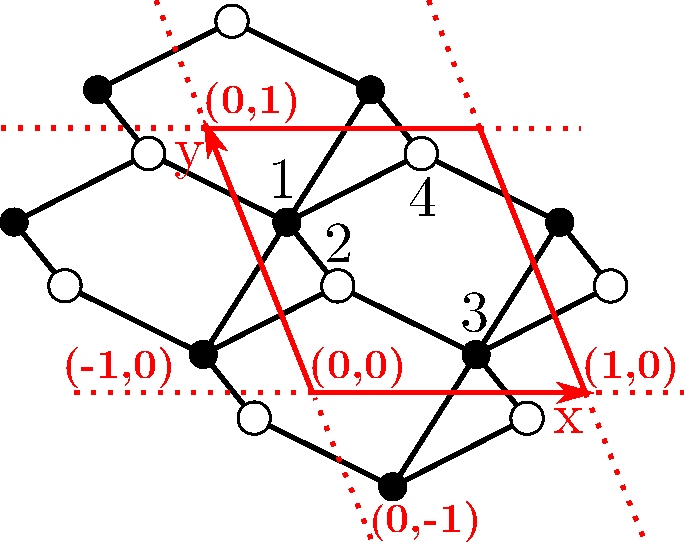
\includegraphics[width=0.63\linewidth]{figures/topology/cells_super.pdf}
		\vspace{-0.5em}
		\subcaption{Non-unit cell}
		
		\centering\scriptsize\begin{tabular}{ccccc}
			1&2&&0&0\\
			1&3&&-1&0\\
			1&3&&0&1\\
			1&4&&-1&0\\
			1&4&&0&0\\
			2&3&&-1&0\\
			2&3&&0&0\\
			3&4&&0&-1
		\end{tabular}
		\vspace{-0.5em}
	\end{subfigure}
	\vspace{2mm}
	\caption{Six different representations of the same 2-periodic graph. The first two columns are the source and destination vertices, the last two are the edge offset.} \label{periodiccells}
\end{figure*}

I implemented the graph structure detailed above in a companion Julia package, \texttt{PeriodicGraphs.jl}, which can be used independently of \texttt{CrystalNets.jl}. That package also contains dedicated ring statistics algorithms, of independent interest for the topological analysis of materials.\\

\Cref{periodiccells} shows several representations of the same 2-periodic graph. The graph is made of two kinds of vertices (represented by open and closed circles), but the choice of the vertex identifiers and of the cell influences the representation. Each choice of cell is characterised by its origin and its axes $x$ and $y$; some repeated cells are represented as well, along with their offset in the bottom-left corner. For each representation, the key is written below, each line referring to a direct edge. Recall that the Systre algorithm works by choosing the lexicographically smallest key from a set of representations, extracted from candidates that do not depend on the representation of the graph. Hence, if the set of representations was those shown in the figure, the topological genome of the graph would be the smallest key, \textit{i.e.} that under representation {\sffamily(a)}.

%The graph structure detailed above was implemented in a new Julia type, \texttt{PeriodicGraph\{N<:Integer\}} whose type parameter \texttt{N} is the space dimension $N$. This type is declared as a subtype of \texttt{AbstractGraphs}, from Julia's \emph{LightGraphs.jl} library. Simply declaring this subtyping relation and implementing a small number of appropriate methods (such as \texttt{neighbours} to collect the neighbours of a vertex, or \texttt{edges} to enumerate the direct edges) makes many of the algorithms implemented in \emph{LightGraphs.jl} natively work for the new type \emph{PeriodicGraphs.jl}.

%An adaptation is required in some cases however. For instance, in order to compute the coordination sequence of a vertex, the algorithm needs an efficient way to store which vertices were already encountered. For a 3-periodic graph, this problem boils down to finding a bijection $h:\Z^3\to\N$ such that
%\[\forall (o_1, o_2)\in(\Z^3)^2,\ \norm{o_1}_1 < \norm{o_2}_1\implies h(o_1) < h(o_2)\]
%Such a function $h$ and its relation to the problem of computing the coordination sequence is detailed in [APPENDIX A].\\

Having a working representation for nets, let's now discuss my reimplementation of the Systre algorithm \autocite{Systre} to compute a unique identifier for each net topology.

%\begin{itemize}
%	\item Specificity of periodicity: neighbour offsets. Distinction between undirected edges and signed offset.
%	\item Summary of the configuration: small to medium-sized graph, very sparse adjacency matrix, need for optimum speed in the computation of neighbours
%	\item Representation of a graph as a list of neighbours. Forbidden loops
%	\item Integration within the LightGraphs ecosystem: free algorithms.
%	\item Special optimisation for the computation of the coordination sequence: unit cell width and hash function.
%\end{itemize}


\subsection{Equilibrium placement}

\subsubsection{Definition}

Given a periodic graph, the first step is to compute, for each vertex $(u,o')\in V\times\Z^3$, a position $p(u,o')\in\R^3$ such that
\begin{equation}
	\forall u\in V,o'\in\Z^3,\ p(u,o') = \frac1{\abs{N_{u}}}\sum_{(v,o)\in N_{u}}p(v,o'+o)
	\label{equilibrium1}
\end{equation}
The set of positions $p$, called an \emph{equilibrium placement}, is such that each vertex is at the barycentre of all its neighbours. $p$ must also satisfy the additional constraint that
\begin{equation}
	\forall u\in V,\ o\in\Z^3,\ p(u,o) = p(u,\OZ) + o
	\label{equilibrium2}
\end{equation}
to enforce the periodicity of the equilibrium placement.

The equilibrium placement has been proven to be unique modulo isometries, because it is the solution of a full-rank linear problem\autocite{barycentric}.
\Cref{equilibrium1} can be rewritten with \cref{equilibrium2} in matrix form, $A\times P = O$, where $A\in\cal M_{n,n}(\Z)$, $O\in\cal M_{n,3}(\Z)$ and unknown $P\in\cal M_{n,3}(\R)$ such that, noting $n(u,v)$ the number of neighbors of $u$ whose identifier is $v$:
\begin{itemize}[noitemsep]
	\item $\forall (u,v)\in V^2,\ A_{u,v} = \begin{disj}{cl}
		\abs{N_u} - n(u,u)&\t{if }u=v\\
		-n(u,v)&\t{otherwise}\\
	\end{disj}$%\mathds1_{u\t{ and }v\t{ are neighbours}}$
	\item $\forall u\in V,\ O_u = \sum\limits_{(v,o)\in N_u}o$
\end{itemize}
and from which we determine for all $u\in V$, $p\left(u, 0_{\Z^3}\right) = P_u$.

Since the coefficient of $A$ and $O$ are integers, the computed solution $P$ is always in $M_{n,3}(\Q)$ with the additional constraint that one of the vertices $u$ be placed at the origin. The exact solution with coefficients in $\Q$ is actually necessary for the subsequent computations and not an approximation, so the resolution of the system must be exact. This turns out to be a very costly operation: it requires storing integers of arbitrary size, which are computationally far more expensive than fixed-width machine integers.

\subsubsection{Computational aspects}

The GNU Multiple Precision Arithmetic Library (GMP) \autocite{GMP} provides access to heavily optimised structures that allow to efficiently perform exact integer and rational computations. Julia has native support for the arbitrarily-sized integer structure from GMP, through the \texttt{BigInt} type, but does not provide a full interface for GMP's rational numbers (although it is internally used for Julia's native \texttt{Rational\{BigInt\}} type). As part of this work, I provide this special support in a separate package, \texttt{BigRationals.jl}, which exports the \texttt{BigRational} type wrapping GMP's rational type.

In addition to the data structure used, a choice has to be made about the algorithm for solving this linear system. The most straightforward idea would be a general linear algebra technique such as LU decomposition followed by forward and backward substitution. Yet, matrix $A$ is structured since it is both symmetric and sparse, calling for the use of more efficient algorithms. %Unfortunately, Julia does not currently have a specialised solver for exact sparse linear systems, it needs to be either an approximate solution or a dense matrix computation, whose cost is prohibitive in large cases.


Several algorithms have been discussed in the literature for the exact resolution of sparse and integer linear systems \autocite{sparseLinearRational,blackbox,Dixon,Wiedemann}. Following the analysis by Eberly \textit{et al.} \autocite{sparseLinearRational}, I decided to implement Dixon's algorithm \autocite{Dixon} which relies on a modulo-prime inversion of the matrix. In accordance with their conclusion, this algorithm largely outperforms a sparse LU decomposition algorithm (which I also implemented as a reference and for benchmarking), both algorithms leveraging GMP instructions specific to the \texttt{BigRational} type for improved performance. Yet, Dixon's algorithm can fail if matrix $A$ happens not to be invertible modulo the chosen prime: hence, I chose to successively invert it modulo three hard-coded large primes and stop at the first succeeding one, and finally resort to LU decomposition if all three fail.
This implementation is up to orders of magnitude faster than that used in the original Systre program written in Java. This extra performance is crucial for the use of the topology detection algorithm as part of large-scale screening methodologies.

% outdated: the current algorithm is Dixon's, much faster than LU.
%To circumvent this issue, we implemented a sparse LU decomposition algorithm that leverages GMP instructions specific to the \texttt{BigRational} type for improved performance. This implementation is faster than that used in the original Systre program, especially for large graphs (with up to 920 vertices for the biggest net of the RCSR database, called {\bf tep}). But better algorithms exist and have been discussed at length in the field of sparse integer linear systems resolution \autocite{sparseLinearRational,blackbox,Dixon,Wiedemann}. %, with techniques such as [modulo-prime reduction] or [floating point approximation], etc.
%I did not have the time to implement those advanced algorithms yet, but plan to in the future.\\

The equilibrium placement naturally embeds the graph in a Euclidean space, namely $\Q^3$. The first vertex of the graph is placed in position $(0,0,0) = \OQ$, which is allowed because any translation of the equilibrium placement still results in an equilibrium placement.
Moreover, because of \cref{equilibrium2}, for any vertex identifier $u\in V$ there is an offset $o$ such that $p(u,o)\in\left[0,1\,\right[^3$, where $\left[a,b\,\right[$ designates the set of reals between $a$ (included) and $b$ (excluded). In order to simplify the representation, this offset is set to $\OZ$ by adjusting the offsets of the edges of the graph accordingly. In this new representation, equations \ref{equilibrium1} and \ref{equilibrium2} still hold, as well as the new property:
\[\forall u\in V,\ p(u)\in \big(\Q\,\cap\,\left[0,1\,\right[\big)^3\quad\t{where }p(u) = p(u,\OZ)\]

In order to accelerate the subsequent algorithms, the vertices of the graph are lexicographically sorted according to their new position. The first vertex, being at $\OQ$, remains first.

Nets where at least two vertices have the same position are called \emph{unstable} and, similarly to Systre, are generally not handled by \texttt{CrystalNets.jl}. This is usually not problematic since their probability of occurrence is low \autocite{unstableNets}. My implementation can however handle unstable nets where each collision site comprises at most four vertices if there is no edge between two different collision sites and no collision site is bonded to two representatives of the same vertex. This accounts for roughly half of the encountered unstable nets in the explored databases. I will not detail the case of these unstable nets here but focus on stable ones, so we can thus assume that no two vertices have the same position.\\
% -> supplementary material?

\Cref{diavmd} represents the equilibrium placement for the net of diamond (called {\bf dia} in the RCSR). Note that the natural embedding in $\Q^3$ imposes a cubic unit cell for all nets, which is not representative of the actual unit cell of diamond; however, the geometry of the unit cell is irrelevant here because only the topology of the net matters. As a consequence, the bond lengths are not representative of that of diamond either, which explains why not all have the same lengths in this representation. Nonetheless, each vertex is indeed at the barycentre of the positions of its neighbours.

\begin{figure}[ht]
	\centering
	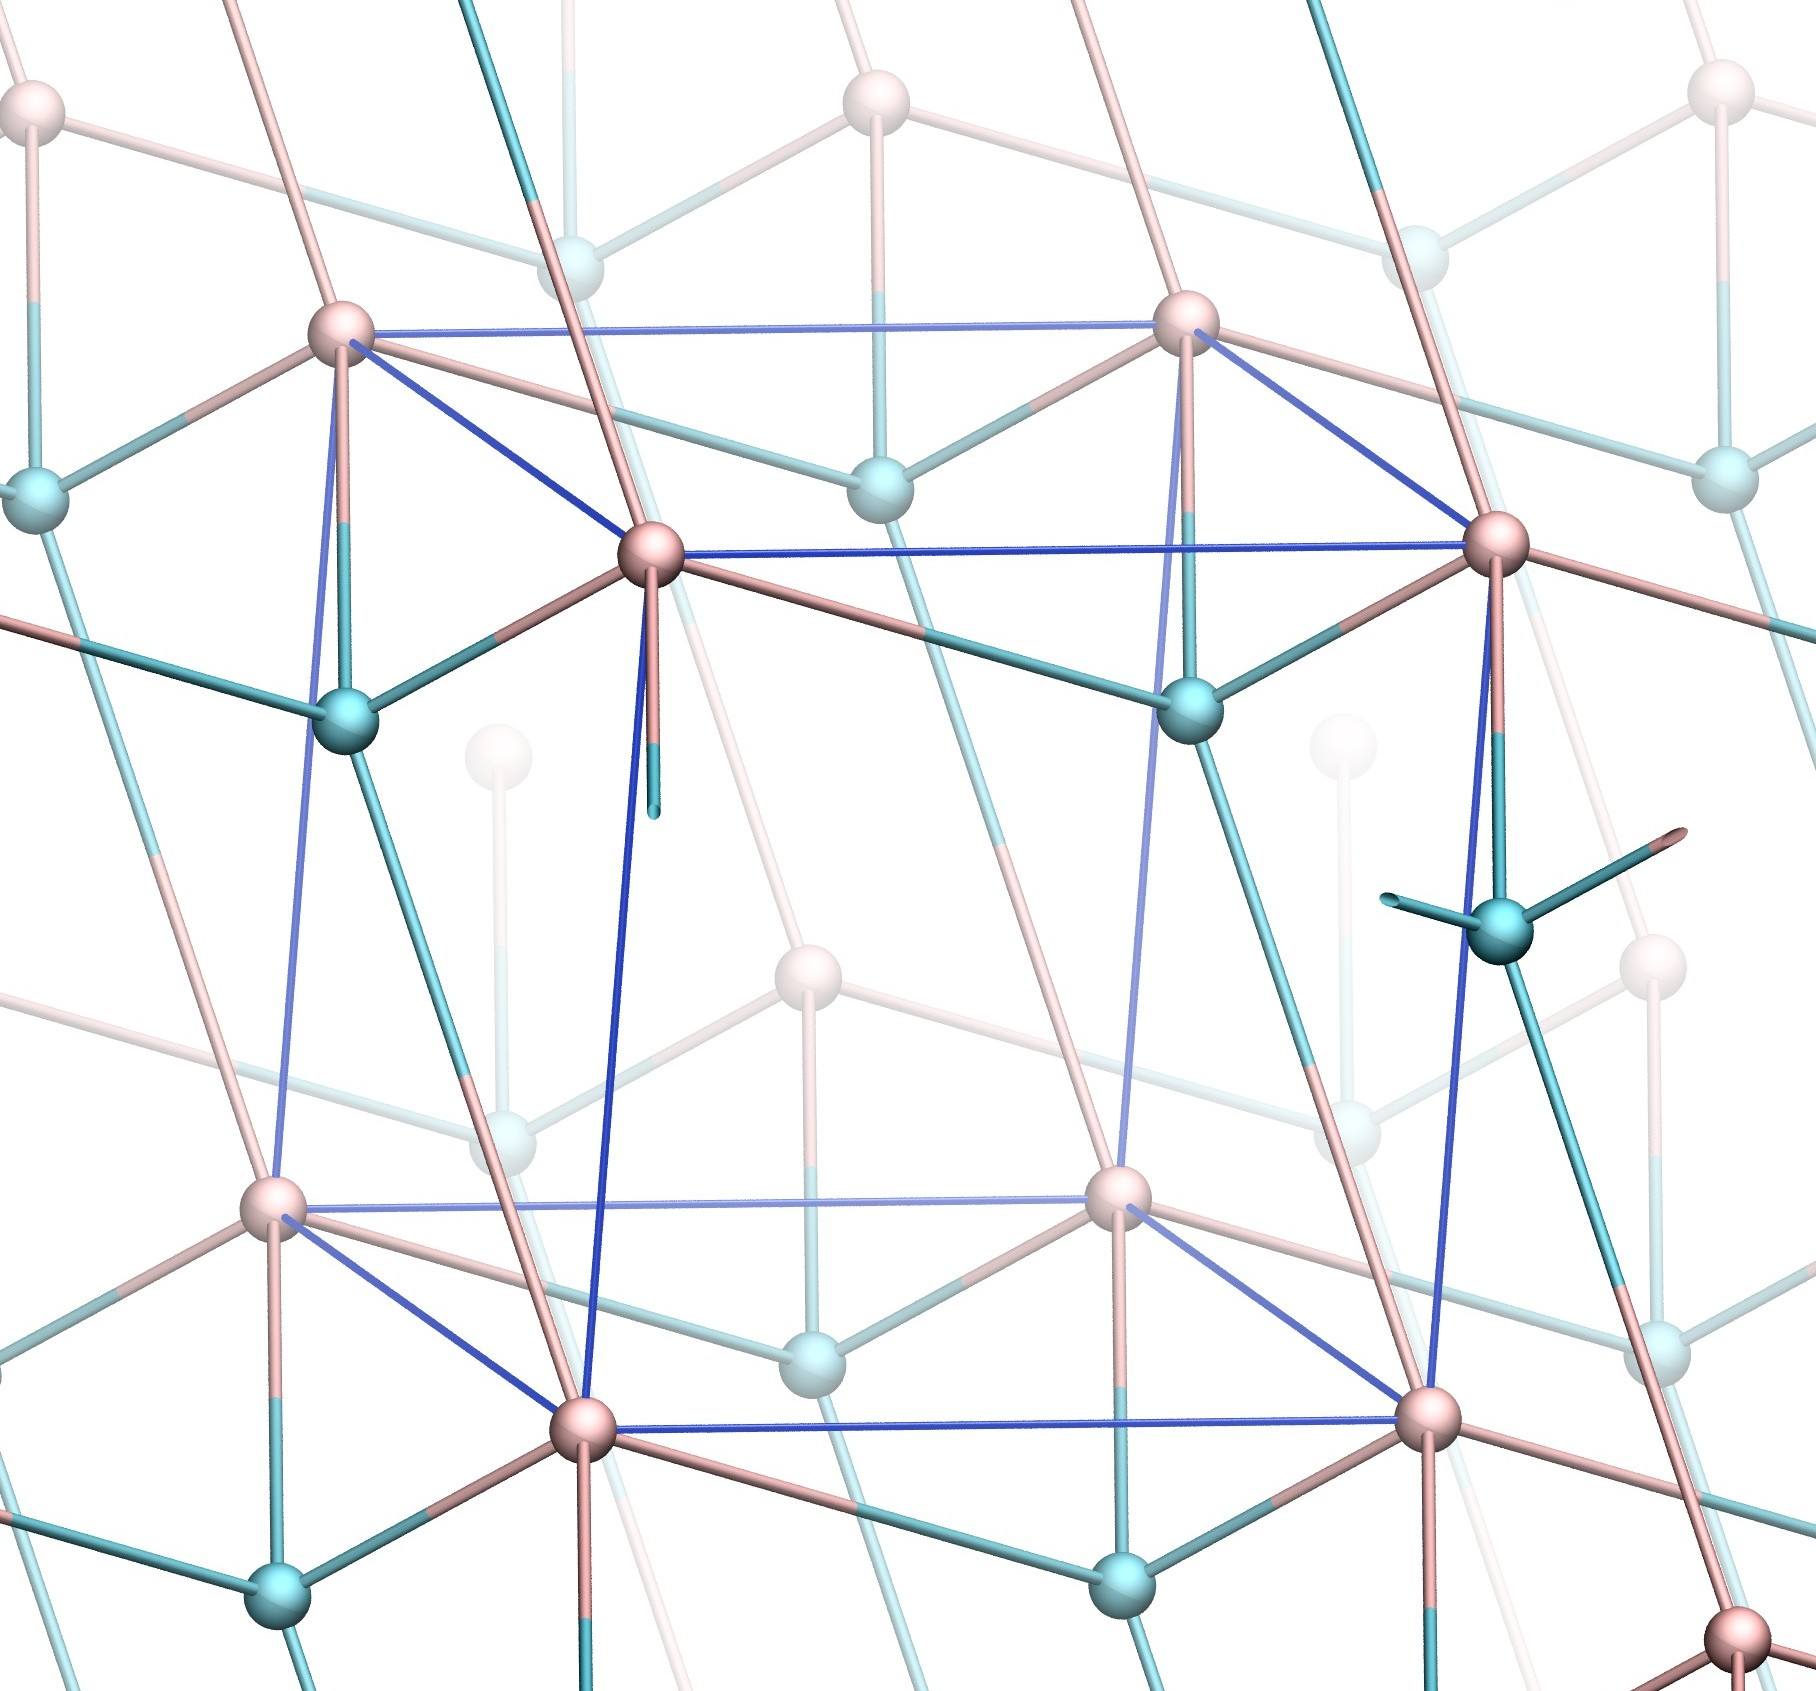
\includegraphics[width=0.4\linewidth]{figures/topology/dia.jpg}
	\caption{Natural Euclidean embedding of the equilibrium placement for the {\bf dia} net.}
	\label{diavmd}
\end{figure}

%\begin{itemize}
%	\item Mathematical definition of the problem and direct resolution
%	\item Implementation note: no prior implementation of sparse resolution for rational matrices.
%	\item BigRational type
%	\item Other possible techniques for future faster resolution
%\end{itemize}


\subsection{Minimisation of the graph}

\label{minimisation}

Once the equilibrium placement is found, the next step of the algorithm is to find a unit cell. In general, a \emph{cell} is a parallelepiped whose three axes $(\vec a, \vec b, \vec c)$ are linearly independent translations that constitute symmetries of the graph. Such translations will be called \emph{valid translations}. Another representation for this cell is the matrix $A$ whose columns are respectively $\vec a$, $\vec b$ and $\vec c$. Its volume is $\det(A) = (\vec a\wedge\vec b)\cdot\vec c$. It is a \emph{unit cell} if it contains the smallest possible number of vertices, which is equivalent to having a minimal volume. %[CITATION].

At this point, it is important to recall that the Euclidean space in which the graph is embedded through the equilibrium placement depends on its initial representation, so there is no simple way of finding a unique unit cell independently of the original representation. In particular, common cell reduction techniques such as Delaunay \autocite{Delaunay} or Niggli \autocite{Niggli, reducedCell}, which yield a uniquely defined cell, do not solve this problem. Unfortunately, existing libraries implementing these techniques (like spglib \autocite{spglib} or cctbx \autocite{cctbx}) cannot be used either for the simpler problem of finding any unit cell because they do not handle arbitrary precision.
%However, different cells can still be compared according to their volume under the condition that they are measured in the same euclidean space. Hence, I look for the unit cell with minimal volume in the initial euclidean space used for the equilibrium positions.
\\

First, note that, by construction of the equilibrium placement, the initial cell is the canonical basis of $\Q^3$, so its matrix is the identity $I$. Let's now assume that $I$ is not a unit cell and there is a unit cell $A\in\Q^{3\times3}$ of volume $\det(A)\in\left]\,0,1\,\right[$.

Let's define $f:\Q\to\Q\cap\left[0,1\,\right[, \displaystyle\frac pq\mapsto\frac{p\%q}q$ where $p\%q$ is the remainder of the euclidean division of $p$ by $q$ (hence $p\%q\in\brack{0,q-1}$). Let $B = \paren{f(A_{i,j})}_{1\le i,j\le3}\in\Q^{3\times3}$. By definition of $f$, the columns of $B$ are axes within the initial cell; moreover, since $\forall x\in\Q,\ x-f(x)\in\Z$, each axis of $B$ can be seen as the corresponding axis of $A$ plus an offset $o\in\Z^3$. But since $I$ is a repeating unit, such an offset is a valid translation, so each axis of $B$ is a valid translation. Finally, since $\det(A)\notin\Z$, not all coefficients of $A$ can be integers, so $A$ has at least one coefficient $x$ such that $f(x)\ne0$, so at least one axis of $B$ is not $\OQ$.

To summarise, the previous observations show that if the initial cell was not a unit cell, then there exists a non-zero valid translation $t\in\big(\Q\,\cap\,[0,1[\big)^3\setminus\{\OQ\}$.\\

Let's use this fact to find a unit cell by enumerating all such translations. Symmetries map vertices to vertices, so the first vertex (lexicographically sorted by position) is mapped to another. But since the first vertex was put in position $\OQ$, the translation is directly given by the position of the other vertex. Hence, only $n-1$ translations need to be checked, and if none is valid then the initial cell is a unit cell.

Checking whether a translation is valid can be done with $O(n\log n)$ time complexity. Vertices are already sorted by position, which allows to efficiently check that all the vertices are mapped to vertices. Doing so first allows to collect the map from initial vertices to their new counterparts and return early if the translation is invalid. Afterwards, it remains to be checked that all edges are also mapped to edges, which can also be done efficiently since the lists of neighbours $N_u$ where $u\in V$ are also lexicographically sorted.

If $I$ is not a unit cell, then a valid translation $t = (t_1,t_2,t_3)\in\big(\Q\,\cap\left[0,1\,\right[\big)^3\setminus\{\OQ\}$ must have been found. Let $k\in\brack{1,3}$ be such that $t_k$ is the smallest non-zero coefficient of $t$. Then a new smaller cell is given by matrix $\der At$ where
\[{\der At}_{i,j} = \begin{disj}{cl}
	t_i &\text{ if } j = k\\
	1&\text{ if } j\ne k\text{ and }i = j\\
	0&\text{ otherwise}
\end{disj}\]
The volume of $\der At$ is $\det(\der At) = t_k\in\left]\,0,1\,\right[$ and by constructions its axes are all valid translations, so $A$ is indeed a new smaller cell. This process can then be iterated in the new Euclidean space created by mapping each point $x\in\Q^3$ to $(\der At)^{-1}x$, until no valid translation is left.\\

There are several ways to improve the computational complexity of this procedure. The first one consists in observing that if $t\in\Q^3$ is a valid translation, then so is $k\times t + o$ where $k\in\Z$ and $o\in\Z^3$. This allows to minimise the volume of the new cell $\der At$ thanks to algebraic considerations. Let's illustrate this point in two dimensions for simplicity, although it can be generalised to any number of dimensions.

Let $t =\paren{\frac{p_1}{q_1}, \frac{p_2}{q_2}}$ be a valid translation. Let's assume that $p_1\ne0$ and $q_1 \ge q_2$ (the opposite reasonning can be done in the other case). Let $k\in\Z$ and $k'\in\Z$ be B\'{e}zout coefficients for $p_1$ and $q_1$, \textit{i.e.} such that $kp_1 + k'q_1 = 1$, and let $o = (k', 0)\in\Z^2$. Then $k\times t + o = \paren{\frac1{q_1}, \frac{kp_2}{q_2}}$.
%$k\times t + o = \paren{\frac{kp_1+k'q_1}{q_1}, \frac{kp_2}{q_2}}$

Hence, matrix $\der A{kt+o}$ can replace $\der At$ to reduce the cell to a volume $\frac1{q_1}$ instead of $\frac{p_1}{q_1}$.\\

Another potential improvement consists in using all the valid translations instead of stopping at the first one encountered. This way, the translation that minimises the volume of the new cell can be chosen instead of any valid translation. However the cost of collecting all valid translations can be up to $n$ times higher than finding the first valid translation.

Furthermore, $\der At$ is just a special case of the set of possible new cells. In general, any invertible matrix whose columns are valid translations (including columns of the identity matrix) is the matrix of a valid cell. The best new cell is the one with the smallest volume, but combinatorial exploration of all possible such matrices that lead to smaller cells has a worst-case complexity of $O(n^3)$. In practice, many candidate matrices can be eliminated before computing their determinant so using this method is actually quite efficient.


%Since $I$ is a unit cell, there are representatives of $u$ in positions $(1,0,0)$, $(0,1,0)$ and $(0,0,1)$. But since $A$ is a unit cell, these positions also correspond to representatives of $u$ at offsets $o_1$, $o_2$ and $o_3$ with respect to unit cell $A$, with $o_i\in\Z^3$ for $i\in\brack{1,3}$. Hence, $A^{-1} = \big[\ o_1\ o_2\ o_3\ \big]\in\Z^{3\times3}$ so $q = \det(A^{-1})\in\Z$. Additionally, the axes of $A$ were chosen in direct order and $A^{-1}$ is invertible so $q\in\N^*$.

% 
%
%The equilibrium placement is an euclidean embedding of the graph, but it still depends on its initial representation. In particular, the number of vertices of the graph is the same as in the original input. The next step of the algorithm consists in finding an isomorphic representation of the graph with the minimum number of vertices.
%
%Reducing the number of vertices consists in finding another unit cell such

%\begin{itemize}
%	\item Search space for reduction
%	\item Matrix formulation
%	\item Incremental reduction vs all-in-one approach
%\end{itemize}

\subsection{Search space exploration}

\begin{figure*}[p]
	\begin{center}
		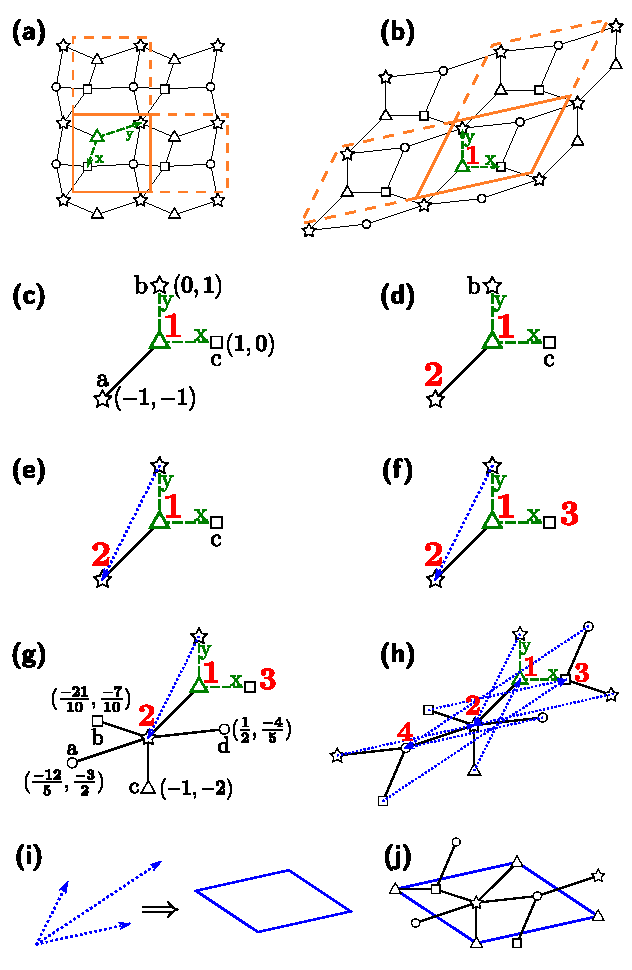
\includegraphics[width=0.9\linewidth]{figures/topology/candidates.pdf}
	\end{center}
	\caption{Illustration of the algorithm used to extract a key from a candidate on a 2-dimensional graph}
\end{figure*}

\begin{figure*}\ContinuedFloat
	\begin{fminipage}{\linewidth}
	\begin{enumerate}[label={\sffamily\small\bfseries(\alph*)},itemsep=0em]
		\item Start from a candidate (in {\color{green!50!black}green}), whose origin is $\boldsymbol\triangle$ and axes are $x$ and $y$. Initialise an empty queue of vertices.
		\item Represent the graph in the basis given by the candidate (the former unit cell and two of its neighbours are represented in {\color{orange}orange}). Note that axes $x$ and $y$ are now orthogonal. Assign number 1 to the origin $\boldsymbol\triangle$ and push it to the queue.
		\item Take the first vertex $u$ of the queue and sort its neighbours according to the lexicographical order of their position. Here, $u = 1$ and the sorted neighbours are a, b and c.
		\item For each neighbour $v'$, in order, if it is not the representative of an already encountered vertex, assign it the first available number between 1 and $n$ and push it to the queue. In this case, neighbour a is assigned number 2.
		\item Otherwise, store the translation between the newly encountered representative $v'$ and that which has been recorded $v$ (the {\color{blue}blue} arrow). Here, $v'$ is neighbour b and $v$ is vertex 2: both are representatives of the same vertex.
		\item Continue until all the neighbours have been processed. In this case, only neighbour c remains and it is assigned number 3.
		\item Repeat the steps from {\sffamily\small\bfseries(c)} until the queue is empty. Here, the neighbours of 2 are being processed.
		\item When the queue is empty, all numbers between 1 and $n$ have been assigned and a set of translations has been recorded.
		\item Triangulate the set of positive translations to obtain a new unit cell (see \cref{triangulate}).
		\item Convert the translations to integer offsets using the unit cell to find a new representation of the graph, and extract the key.
	\end{enumerate}
	\vspace{8mm}
	
	\caption{\emph{Continued:} Illustration of the algorithm used to extract a key from a candidate on a 2-dimensional graph} \label{algocandidate}
	\end{fminipage}
\end{figure*}


At this stage in the workflow, the graph has a unit cell and a corresponding equilibrium placement. Let's now look for the topological genome. The strategy follows that implemented in Systre, which consists in taking the lexicographically smallest key among those computed for a number of candidates. Both the computation of the key from a given candidate and the selection of the candidates should not depend on the current representation of the graph.

A candidate is defined as a triplet of linearly independent edges, and represented by a pair \{vertex, basis of $\Q^3$\} where the vertex is the source of the first edge and the columns of the basis are the translations induced by the edges. The process of selecting candidates is explained in \cref{searchspacereduction}. This subsection focuses on the computation of a key from a given candidate.\\

\label{searchspaceexploration}

This precise algorithm is explained in \cite{Systre} and analysed as Algorithm 5 in \cite{barycentric}. It is detailed in \cref{algocandidate}. The main point is that the algorithm creates a new representation of the graph which is independent of the previous one by redefining both the unit cell and the numbering of vertices thanks to a unique euclidean space derived from the candidate. The first element of the candidate, the vertex, is the origin of the new space and the columns of the basis are its three axes.
%In this space, a queue of vertices is initialised with the origin, which gets the new number $1$. Then, at each successive step of the algorithm, the first element $u$ of the queue is taken and its neighbours are sorted by lexicographical order of their position in the new euclidean space. Note that this ordering is independent of the initial representation, it only depends on the new space, hence on the candidate. For each neighbour of $u$ taken in order, there are two possibilities:
%\begin{itemize}[noitemsep]
%	\item either the neighbour is a representative $v'$ of a vertex whose new number $v$ has already been assigned. In that case, the edge $(u,v,t)\in V\times V\times\Q^3$ is stored where $t\in\Q^3$ is the translation between the position of $v$ and that of its representative $v'$.
%	\item otherwise, it means that none of its representatives has been processed yet. In that case, let's assign it the first available number $v$ between $1$ and $n$, push $v$ to the queue and store the edge $(u,v,\OQ)$.
%\end{itemize}

Step {\sffamily\small\bfseries(b)} is a simple affine transformation of the positions and steps {\sffamily\small\bfseries(c)} to {\sffamily\small\bfseries(h)} are straightforward to implement, they only require keeping track of the positions of the numbered vertices. Step {\sffamily\small\bfseries(j)} is also straightforward, it consists in multiplying each translation by the inverse of the matrix of the new unit cell to obtain an integer offset. This allows to retrieve the set of edges $E$ of the graph, and since $V = \brack{1,n}$, this directly yields the representation of a periodic graph in the vector model.

\phantomsection
\label{triangulate}

Step {\sffamily\small\bfseries(i)} deserves special consideration. It consists in building a new unit cell from the set of positive translations $t$ of the edges, positive in the sense of being lexicographically greater than $\OQ$. Negative translations are negated to only keep positive ones. By construction, this set does not depend on the previous representation of the graph, it only depends on the candidate. As a consequence, any deterministic algorithm that transforms a set of translations into a unit cell can be used for this purpose. Delgado-Friedrichs and O'Keeffe \autocite{Systre} mention this point and suggest triangulating the translations, without detailing their algorithm. Before presenting the one used here, let's sketch the general idea and prove a lemma.\\

Given their origin, translations of the set should correspond to integer offsets between vertices and their representatives in the new unit cell to be found. Thus, the matrix $B\in\Q^{3\times3}$ representing the unit cell must be such that each positive translation $t\in\Q^3$ of the set verifies:
\begin{equation}
	B^{-1}t = o\in\Z^3
	\label{unitcellcondition}
\end{equation}
Not all such basis $B$ will do, since it should also represent a unit cell, hence the columns of $B$ must be valid translations. Since all positive translations of the set map some vertex to one of its representatives, they are all valid translations, so it is tempting to look among the integer combinations of these translations to find the columns of $B$. However, it remains to be proven that such combinations indeed span the entire group of valid translations.

To show this, let's take the Euclidean space of step {\sffamily\small\bfseries(b)} and consider a path between the origin and any of its representatives. This path consists in a series of edges $(u,v,t)\in V\times V\times\Q^3$ where $t$ is the translation between vertex $v$ and the vertex $v'$ which is the actual neighbour of $u$. After any number of steps, let's note $(u,\tau)\in V\times\Q^3$ the pair where $u$ is identifier of the vertex on which the path has just landed and $\tau$ is the sum of the translations $t$ encountered so far. The initial pair thus is $(1,\OQ)$, since $1$ is the number of the origin. An induction on the number of steps shows that the position of the exact vertex on which the path lands when reaching pair $(u,\tau)$ is that of vertex $u$ translated by $\tau$. As a consequence, when reaching the final vertex of the path, the pair is $(u_\t{end},\tau_\t{end}) = (1,\tau_\t{end})$. Thus, by construction $\tau_\t{end}$ is the sum of translations $t$ stored in the edges during the algorithm, so it is an integer combination of the positive translations of the set. But since this reasoning was valid for the translation between the origin and any of its representatives, this proves that any valid translation can be written as an integer combination of positive translations of the set.\\

Let's now proceed to the algorithm that converts the set of positive translations into a matrix $B$ satisfying \cref{unitcellcondition}.

First, note that most positive offsets present in the usual representations of periodic graphs are one of either $(1,0,0)$, $(0,1,0)$ or $(0,0,1)$. As a consequence, in the most common cases, there are only three elements in the set of positive translations, which can simply be mapped to the three canonical offsets. This fact serves as a heuristic optimisation for the more general algorithm, by representing all the positive translations in the basis $A\in\Q^{3\times3}$ whose columns are the three first linearly independent positive translations. The reverse transformation will be applied at the end of the algorithm. Overall, this operation is not crucial for the algorithm to work and the input remains a set of translations, but it tends to reduce the denominators of the coefficients of the translations, which is computationally helpful.

Given a set of translations, the goal now is to find three combinations such that they form the columns of a matrix $B$ satisfying \cref{unitcellcondition}. In other words, these combinations must span the group of valid translations. This problem on rationals is lifted to integers by storing the least common multiple of the denominators of the coefficients of the translations columnwise, and pointwise multiplying the translations by this triplet of integers in order to obtain a set of integer translations.

From that point, several algorithms exist in order to solve the problem on this integer form \autocite{sparseLinearRational,blackbox,Dixon,Wiedemann}. The standard procedure is to build the rectangular matrix whose lines are the triplets representing integer translations and put it in Hermite normal form \autocite{gcd}, which is precisely such that it is built from an integer combination of the initial triplets and still spans the same group as that of the triplets.

Determining the exact Hermite normal form is useless in this case however, since there is no need for the complexity brought by its other properties, and the existing solvers are specialised to have their best performance on big square matrices, not thin rectangular matrices one of its dimensions being only 3. Thus, I implemented a custom solver for this particular problem which performs the following steps, for each column $j$ in a fixed order:
\begin{itemize}[noitemsep]
	\item Find B\'{e}zout coefficients of the $j$-th element of the integer translations, as well as their greatest common divisor $d\in\N^*$. This is done using an efficient algorithm from Havas \textit{et al.} \autocite{gcd}.
	\item Set the $j$-th column of $B$ as the sum of the integer translations weighted by their B\'{e}zout coefficient. %By construction, this new column will have $d$ as its $j$-th element and zeros afterwards, so that $B$ will be lower triangular.
	\item For each integer translation $t\in\Z^3$, update it to zero its $j$-th element by subtracting the new column of $B$ times the quotient of the $j$-th element of $t$ by $d$. By construction, after this step all translations have at most $(j-1)$ non-zero elements.
\end{itemize}
Finally, columnwise divide $B$ by the triplet of least common multiples that was found before to get back to rationals, and left-multiply it by $A$ to go back to the Euclidean space specified by the candidate.\\

The resulting matrix $B$ has all the required properties for being a unit cell. Thus, each translation $t\in\Q^3$ of an edge now corresponds to an offset $o = B^{-1}t\in\Z^3$ with respect to the unit cell, so the lexicographically ordered set of edges $(u,v,o)\in V\times V\times\Z^3$ is a representation of the initial graph that does not depend on its initial representation, but only on the candidate.

Let's note that this method transforms a set of translations into a unit cell, and this is precisely the problem encountered when minimising the cell from the set of all valid translations in \cref{minimisation}. However, in the current case, the procedure cannot rely on a starting cell to minimise, which is why it is more complex.

To conclude, let's observe that this representation might be impossible to embed, in the sense it may be impossible to put all the vertices of the graph, as they were determined by the algorithm, within the same unit cell given the constraints on their edges. This can be circumvented by taking appropriate representatives for each vertex given a fixed unit cell, but even that is unnecessary since the goal is only to extract a key, and it does not matter whether the key itself can be embedded.

% A note on impossible deformation (some representation might be impossible to embed, but it doesn't matter)


%------------------------------------------------

\section{Reduction of the search space}

\label{searchspacereduction}

The only aspect of the algorithm that remains to be explored is the selection of the candidates, which is a crucial point for the overall complexity of the algorithm. After explaining how the implementation of Systre does this, I will present a series of novel reductions of the search space, \textit{i.e.} of the number of candidates, that yield a notable performance gain.

\subsection{The initial search space}

Let's recall that a candidate is defined as a triplet of edges, which is used to create a new representation for the graph as explained in \cref{algocandidate}. The topological genome is chosen as the lexicographically smallest key extracted from the candidates, so the set of candidates must be chosen in a fashion that is independent of the initial representation of the graph, lest the selection biases the search space. As a consequence, Delgado-Friedrichs and O'Keeffe \autocite{Systre} proposed the following selection pattern:
\begin{itemize}[noitemsep]
	\item If there exists at least one vertex such that its outgoing edges are not all coplanar, then the set of candidates is the set of triplets of linearly independent edges that all start at the same vertex.
	\item Otherwise, the candidates are all triplets of linearly independent edges such that the two first start from a common vertex and the third starts from another vertex.
\end{itemize}

In both cases, the set of valid candidates is not empty (otherwise it would mean that the graph is either not connected or not 3-periodic) and independent of the initial representation of the graph. It can be further reduced by removing duplicate candidates that yield the same key, using symmetry considerations as will be shown in \cref{symmetries}.

%Depending on whether all vertices have coplanar neighbours:
%\begin{itemize}
%	\item If not so, then all vertices that do not have all their neighbours coplanar and all triplet of edges that start from the same vertex and are not coplanar
%	\item Otherwise, take $v$ to be any vertex, $e_1$ and $e_2$ any two edges starting from $v$ and $e_3$ any edge such that $\left|e_1\ e_2\ e_3\right|\ne 0$.
%\end{itemize}

For many graphs, this search space remains rather large compared to the set of all possible triplets of edges.  %Nonetheless the computation of the topological genome can still be done in under a minute for most cases, and in a few minutes for the biggest nets in the RCSR database. 
My goal in this project was for this software to be able to tackle very big structures very efficiently, for two different types of applications: high-throughput screening of hypothetical materials, where the topological detection is performed on hundreds of thousands (and sometimes several millions) of structures \autocite{ren2022highthroughput}, and application to very large periodic structures, such as models of amorphous framework materials \autocite{castel2022atomistic}. Therefore, reducing this search space is crucial for performance since it directly tackles one of the bottlenecks in the original implementation of Systre.

\subsection{Categorisation of vertices and edges}

Since the search space must remain independent of the representation of the graph, it can only depend on some properties that are common to all its representations. Such a property is called a \emph{topological invariant}. The only invariant used so far is whether there exists a vertex whose outgoing edges are not all coplanar, but many other invariants exist, such as the three used by ToposPro \autocite{ToposPro}. These properties can be used to considerably reduce the search space by separating vertices according to them.

The core idea of vertex categorisation consists in trying to separate vertices into as many categories as possible, each of these categories being identifiable independently of the representation of the graph. For instance, in this work, vertices are separated according to their coordination sequence (the number of vertices at distance $k$ from the vertex of interest with $k=1,2,...$, see \hyperref[coordinationsequence]{Introduction}), so that two vertices are in the same category if and only if they share the same coordination sequence up to distance 10.%I have not included the computation of the ring numbers yet because it was more involved than the coordination sequences, but it could be used as well to make finer categories.

Vertex categories are then sorted by the total number of outgoing edges from vertices in that category and, in case of equality, by the invariant they were defined from. For example, in our case, ties are broken by lexicographically sorting according to the coordination sequences.% Note again that this does not depend on any precise representation of the graph.

%Now that the categories are defined and sorted, let's look for candidates and try to minimise their number. The following strategy can be used:
%\begin{itemize}[noitemsep]
%	\item Taking the categories in order, stop at the first one such that it has a vertex whose outgoing edges are not all coplanar. If there is such a category, then the candidates are the triplets of linearly independent edges that all start at one vertex of the found category.
%	\item If there is no such category, loop over all the categories in order. For each category $c$, loop over all the other categories in order. Stop if there is a vertex $u$ from category $c$ and an edge $e$ from the other category $c'$ such that there exists two outgoing edges from $u$ that are not coplanar with $e$. The candidates are then all the triplet of linearly independent edges, such that the two first start from the same vertex in the category $c$ and the third starts from a vertex in category $c'$.
%\end{itemize}
%
%\begin{itemize}
%	\item Not all vertices are identical and some of their properties do not depend on their representation. For instance, their degree.
%	\item Recall ToposPro : coordination sequence and ring number. So far, I only focus on coordination sequence because it does not cost much but in the future it might be worth trying to further narrow the categories.
%	\item Categories sorted according to the total number of outgoing edges. [Not modulo symmetries because the symmetry computation could be not exact. Should be fixed by having exact symmetry computation]
%\end{itemize}

With these sorted categories in mind, let's look for candidates and try to minimise their number. The following strategy is used in the improved algorithm:
\begin{itemize}[noitemsep]
	\item Let $c$ be the first vertex category such that there is a triplet of non-coplanar edges starting from the same vertex in $c$ (if no such category exists, skip to the alternative below). Then, for all such triplets, let $c_1$, $c_2$ and $c_3$ be the sorted categories of the vertices to which the initial vertex is bonded with these edges. There are four subsets of such triplets, characterised by whether they satisfy:
	\begin{enumerate}[noitemsep]
		\item $c_1 = c_2 = c_3$.
		\item $c_1 < c_2 = c_3$.
		\item $c_1 = c_2 < c_3$.
		\item $c_1 < c_2 < c_3$.
	\end{enumerate}
	Then the candidates are all the triplets of edges whose categories are in the last non-empty such subset with $(c_1,c_2,c_3)$ lexicographically minimal.
	
	This strategy illustrated for the 2D case in \cref{candidateselection}.
	
	\begin{figure*}[p]
		\begin{center}
			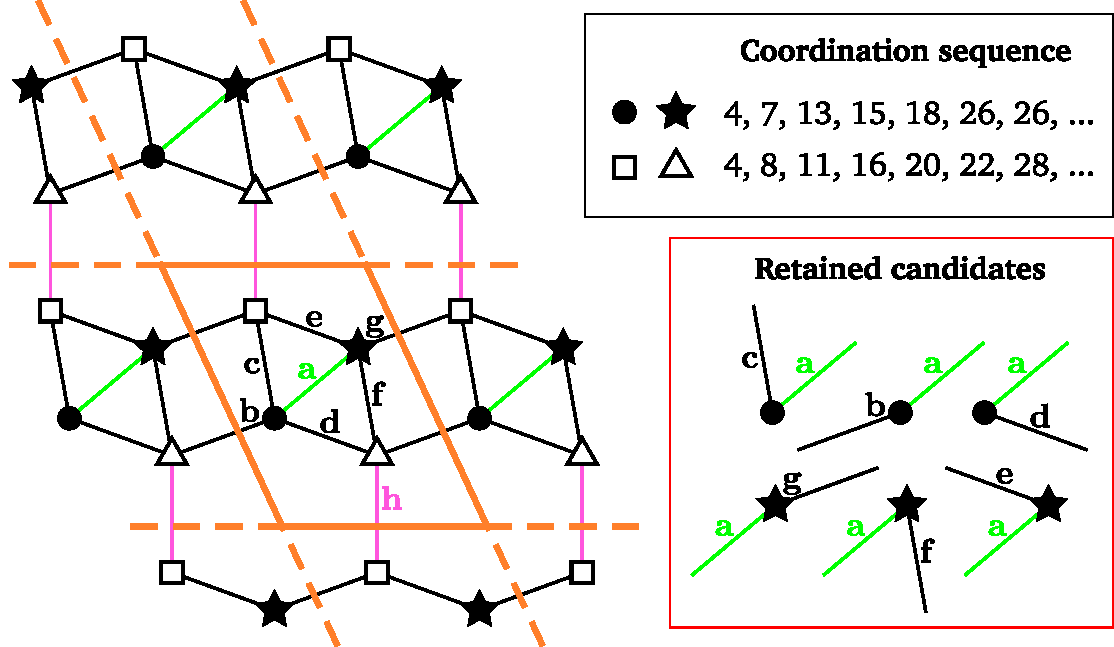
\includegraphics[width=0.79\linewidth]{figures/topology/spacereduction.pdf}
		\end{center}
		\begin{enumerate}[itemsep=0pt]
			\item The coordination sequence of all vertices is computed. In this particular case, there are two vertex categories, one represented with filled symbols (circle and star) and the other with empty symbols (square and triangle). Edges are colored in {\color{green}green} when they connect two filled symbols, in {\color{freespeechmagenta}magenta} for two empty symbols and black otherwise.
			\item Both categories have the same number of outgoing edges, so they are sorted in lexicographical order of the coordination sequences: the ``filled'' category comes first.
			\item There exists a filled vertex with two linearly independent outgoing edges (here, all vertices actually match the criterion because no two neighboring edges are aligned). Hence, $c$ is the ``filled'' category.
			\item Consider all ordered pairs of linearly independent edges starting from a filled symbol $u$. There are 24 such pre-candidates, represented as the two first lines of \cref{allcandidates}. Among those, only 6 bond $u$ to vertices of category $c_1$ and $c_2$ respectively, such that $c_1 < c_2$. Keep those as candidates.
			
			If there was no such pre-candidate, the candidates would have been all the pre-candidates where $c_1 = c_2$ with $c_1$ minimal, \textit{i.e.} ``filled'' if possible, ``empty'' otherwise.
		\end{enumerate}
		\caption{Illustration of the candidate selection on the {\bf cqe} net.}
		\label{candidateselection}
	\end{figure*}
	
	\begin{figure*}[p]
		\begin{center}
			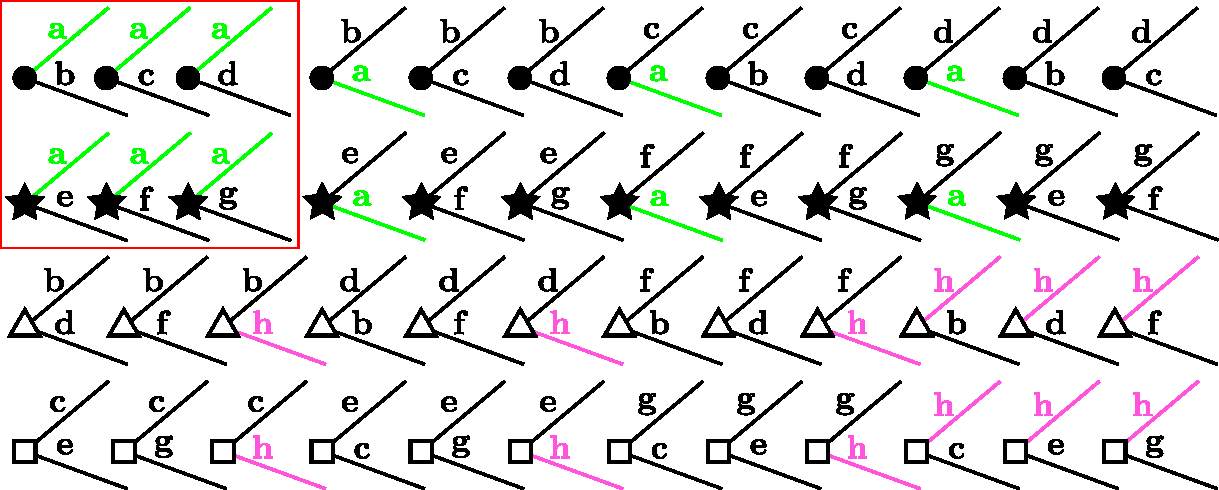
\includegraphics[width=0.88\linewidth]{figures/topology/allcandidates.pdf}
		\end{center}
		\caption{The 6 candidates of the {\bf cqe} net selected by \texttt{CrystalNets.jl}, among the 48 possible candidates.} \label{allcandidates}
	\end{figure*}
	
	\item Alternatively, if all vertices have only coplanar outgoing edges, let $c$ be the first category such that there exists another category $c'$ such that there is a non-coplanar triplet of edges, the two first of which start from a vertex of $c$ and the last from $c'$. $c'$ is chosen as the first such category. Let $c_1$, and $c_2$ be the sorted categories of the destinations of the two first vertices, and $c_3$ be the destination of the third. Then the candidates are all the triplets of edges, the two first of which start in $c$ and the last from $c'$ such that $(c_1,c_2,c_3)$ is lexicographically minimal.
\end{itemize}

The main difference with the strategy of Systre is that the categorisation of vertices bounds the number of candidates with respect to the maximal size of a category, hence the goal of having as many small categories as possible. However, the two strategies are exactly the same in the worst-case scenario where there is only one category. Note that, although rather complex, the constraints on the retained candidates described above can actually be implemented in an efficient way, which is necessary to prevent the search space reduction from taking more time than the actual search space exploration.



%\subsection{Ordering of edge patterns}
%
%A further refinement of the idea of categorisation consists in classifying edges instead of only vertices. Fortunately, the initial categories presented above can be used for this too, by classifying edges with the categories of both their source and destination. The updated strategy becomes the following:
%\begin{itemize}[noitemsep]
%	\item Like before, let $c$ be the first category (if it exists) such that there is a triplet of non-coplanar edges starting from the same vertex in $c$. Then, for all such triplets, let $c_1$, $c_2$ and $c_3$ be the sorted categories of the vertices to which the initial vertex is bonded with these edges. There are four subsets of such triplets, characterised by whether they satisfy:
%	\begin{enumerate}[noitemsep]
	%		\item $c_1 = c_2 = c_3$.
	%		\item $c_1 < c_2 = c_3$.
	%		\item $c_1 = c_2 < c_3$.
	%		\item $c_1 < c_2 < c_3$.
	%	\end{enumerate}
%	Then the candidates are all the triplets in the last non-empty  subset such that $(c_1,c_2,c_3)$ is lexicographically minimal.
%	
%	\item Similarly, if there is no such category, let $c$ be the first category such that there exists another category $c'$ such that there is a non-coplanar triplet of edges, the two first of which start from a vertex of $c$ and the last from $c'$. $c'$ is chosen as the first such category. Let $c_1$, and $c_2$ be the sorted categories of the destinations of the two first vertices, and $c_3$ be the destination of the third. Then the candidates are all the triplets of edges, the two first of which start in $c$ and the last from $c'$ such that $(c_1,c_2,c_3)$ is lexicographically minimal.
%\end{itemize}
%
%Once again, there is no improvement in the worst-case scenario where all the vertices are in the same category. But in all the other cases, this can further minimise the search space. Note that, although rather complex, the constraints on the kept candidates described above can actually be implemented in an efficient way, which is necessary to prevent the search space reduction from taking more time than the actual search space exploration. I implemented a multithreaded algorithm to handle the first case, which further reduces the time taken by this procedure.
%
%\begin{enumerate}
%	\item Taking all the categories in order, if one is such that not all vertices have their neighbours coplanar, then take them and all their triplet of edges that start from $v$.
%	\item Otherwise, for each categories in order, try and see it two edges from $v$ and one other edge, all three within the same category works.
%	\item Otherwise, for each category in order, take two edges from $v$ in that category and one edge from the first other category for which it works. [Note: might be worth checking if removing the second option makes it faster?]
%\end{enumerate}

\subsection{Reduction through symmetry}
\label{symmetries}

In addition to the individual properties of vertices which are used to separate them into categories, symmetry considerations on the equilibrium placement can be useful in reducing the search space. Indeed, if two candidates are symmetry-related, then the representations extracted from both will be exactly identical. This optimisation is already used in Systre, and in the current work, it is useful to perform a symmetry analysis on the equilibrium placement of the unit cell before even categorising vertices.

Unfortunately, there does not appear to be any available code that can find symmetries for an input given in arbitrary precision; all existing libraries take approximate positions, and thus return only approximate symmetries. I use the \textit{spglib} library \autocite{spglib} to this purpose. \textit{spglib} is a C library, which makes it easy to interface with Julia without sacrificing speed. Since all its inputs and outputs are approximate, the returned symmetries need to be checked against the exact equilibrium placement of the graph to rule out false positives. Because of the imprecision of the input, there might also be some false negatives -- that is, some symmetries may be missing -- but they do not matter because symmetries can only help to eliminate candidates that are symmetric images of other ones already encountered. Hence, the use of symmetries is purely an optimisation, but it has no influence on the result of the algorithm. %Having a guarantee that all exact symmetries were found could potentially be useful in order to ... ?

Symmetries are useful to avoid needlessly recomputing coordination sequences when dividing the vertices into categories. Indeed, the search space is reduced by singling out one vertex per symmetry orbit, and using the convention that only these can serve as the source of the first edge of a candidate. No such constraint can be placed on the destinations of the edges unfortunately, as that would be unsound.

On the particular example of the \textbf{cqe} net shown in \cref{candidateselection}, there is only one symmetry and it maps each symbol of a category on the other of the same category. As a consequence, only one of the two first lines and one of the two last lines of candidates shown in \cref{allcandidates} need to be kept. Systre thus examines 24 candidates, and only 3 for \texttt{CrystalNets.jl}.

%In each category, only one vertex is kept per symmetry orbit when computing triplets of edges starting at the same position. For the second case, \textit{i.e.} for triplets of edges only two of which start at the same vertex, this first vertex must also be the only one of its symmetric orbit to be used in this place. There is no such constraint for the source of the third edge and, in both cases, for the destination of any edge, because that would be unsound.

% A note on chirality?

\subsection{Ordering of keys}

Finally, the algorithm can be made faster by changing the mode of comparison of the candidates. In Systre, the topological genome was defined as the smallest key extracted from a candidate. However, arrived at step {\bf (h)} of the algorithm in \cref{algocandidate}, both the embedding of the graph as well as the ordering of its vertices only depend on the candidate. Hence, it is possible to define at that point a pseudo-key consisting in the sorted list of triplets $(s, d, t)\in V\times V\times\Q^3$ if there is an edge between the vertex defined by its number $s$ and the representative of vertex number $d$ which is translated from the latter by $t$. This pseudo-key only depends on the intermediate representation of the graph obtained in step {\bf (h)}, which means it is exclusively determined by the candidate, so the genome can be defined as the key extracted from the candidate with the smallest pseudo-key.

Instead of comparing the keys extracted after a costly lifting of the positive translations to a proper representation of the graph, it is thus sufficient to compare the pseudo-keys. Moreover, this pseudo-key can be computed incrementally during the main loop of the algorithm. To do so, at step {\bf (c)}, the neighbours of vertex $u$ should be sorted in a different manner (represented on \cref{neighbourreordering}): all representatives of the same vertex should be contiguous and lexicographically sorted according to their position within each category; the categories corresponding to vertices which have a number (assigned in step {\bf (d)}) are placed first and sorted according to this number, while the others are placed afterwards and sorted according to the position of the first vertex in the category. This makes it so that each edge of the graph is added to the pseudo-key in the order in which it is studied (in steps {\bf (d)} -- {\bf (f)}), while preserving the invariant that the pseudo-key is lexicographically sorted.

\begin{figure}[t]
	\centering
	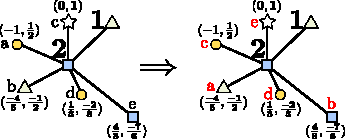
\includegraphics[width=0.85\linewidth]{figures/topology/pseudokey.pdf}
	\caption{Difference between previous and new ordering of neighbours at step {\bf (c)} on an example. Representatives of the same vertex have the same symbol.}
	\label{neighbourreordering}
\end{figure}

Since the pseudo-key is constructed on-the-fly, it can thus be compared at each step with the previous smallest pseudo-key. If a triplet of the current pseudo-key is lexicographically greater than the triplet at the same position in the previous best pseudo-key, the computation for the candidate is aborted; if it is lower then this comparison can be skipped for the rest of the computation and the pseudo-key will be the new smallest. Finally, once all the candidates have been checked, the minimal pseudo-key is converted to an actual key through steps {\bf (i)} and {\bf (j)}, yielding the topological genome of the graph.

%not using the lexicographical order to sort the keys. Indeed, let's order two keys, which are lexicographically ordered lists of edges $(u,v,o)\in V\times V\times\Z^3$, according to the lexicographical order of their source and destination without any offset, and then only, to break ties, according to the offset.
%
%The difference in semantics is illustrated in \cref{orderings}.
%
%\begin{figure}[bh]
%	\begin{subfigure}{0.5\linewidth}
	%		\centering
	%		\subcaption{Lexicographical ordering}
	%		\begin{tabular}{c@{ }c@{\hspace{0.4em}}c@{ }c@{ }c@{ }c}
		%			\color{teal}1&\color{teal}2&&\color{teal}0&\bf\color{orange}0&0\\
		%			1&3&&0&1&0
		%		\end{tabular}\hspace{0.5em}$\bm<$\hspace{0.5em}%
	%		\begin{tabular}{c@{ }c@{\hspace{0.4em}}c@{ }c@{ }c@{ }c}
		%			\color{teal}1&\color{teal}2&&\color{teal}0&\bf\color{orange}1&0\\
		%			1&2&&1&0&0
		%		\end{tabular}
	%	\end{subfigure}\vrule%
%	\begin{subfigure}{0.5\linewidth}
	%		\centering
	%		\subcaption{New ordering}
	%		\begin{tabular}{c@{ }c@{\hspace{0.4em}}c@{ }c@{ }c@{ }c}
		%			\color{teal}1&\color{teal}2&&0&0&0\\
		%			\color{teal}1&\bf\color{orange}3&&0&1&0
		%		\end{tabular}\hspace{0.5em}$\bm>$\hspace{0.5em}%
	%		\begin{tabular}{c@{ }c@{\hspace{0.4em}}c@{ }c@{ }c@{ }c}
		%			\color{teal}1&\color{teal}2&&0&1&0\\
		%			\color{teal}1&\bf\color{orange}2&&1&0&0
		%		\end{tabular}
	%	\end{subfigure}
%	
%	{\vspace{1.5em}\color{teal}Teal}: values compared equal.
%	\\{\bf \color{orange}Bold orange}: values compared different.
%	\\Black: values not compared.
%	\caption{Illustration of the two orderings}
%	\label{orderings}
%\end{figure}
%
%The interest of this choice is that it allows to quickly stop analysing a candidate as soon as it can be shown that the induced key will be sorted after the currently-best key. In particular, since the new ordering initially disregards the offsets of the edges of the graph, it becomes possible to stop before having to lift the rational translations to integer offsets, which is a costly operation.

%------------------------------------------------


\section{Application to materials databases}

\texttt{CrystalNets.jl} is a Julia package which can be intuitively used from an interactive Julia shell or as an executable to determine the structure of single crystallographic files in the variety of file formats recognised by chemfiles\footnote{full list available at \url{https://chemfiles.org/chemfiles/latest/formats.html\#list-of-supported-formats}}. Since chemical bonds are not systematically present in such files, it uses a custom bond detection algorithm inspired from that of chemfiles, and can export both the input with the detected bonds as well as the extracted underlying net to allow visually checking the correspondence with the input. The bonding algorithm reuses available information on the structure to accurately account for the larger bonds surrounding metals in MOFs for instance, but the user can also override the cutoff distance for bonding if necessary.

By combining the bond detection heuristic with topology determination, \texttt{CrystalNets.jl} can also be used to survey large databases of crystalline structures, without the need for user input or relying on other chemical information (such as choice of SBUs) on the structures themselves. In this section, the code is demonstrated on a series of available materials databases.

\subsection{RCSR, EPINET and IZA-SC database}

The Reticular Chemistry Structure Resource (RCSR) \autocite{RCSR} \footnote{available online at \url{http://rcsr.anu.edu.au/nets} (3D) and \url{http://rcsr.anu.edu.au/layers} (2D)} is a repository of 3,132 structures with 2 or 3-periodicity (excluding weaving and 0- and 1-periodic structures), each given a canonical name. It offers a Systre archive containing 2,928 nets that I reprocessed to obtain the 2,928 topological keys corresponding to each structure. These keys are not the same as those of the archive because of the algorithmic differences explained before.

\begin{figure}[t]
	\centering
	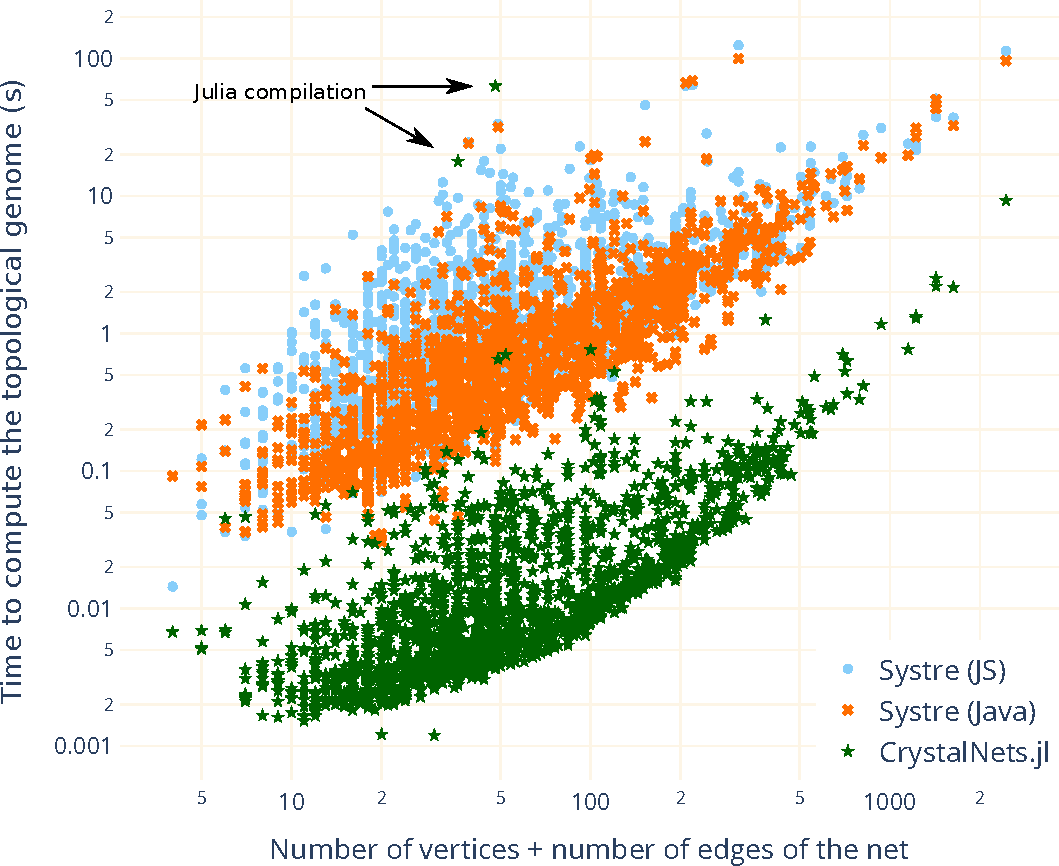
\includegraphics[width=\linewidth]{figures/topology/timings.pdf}
	\caption{\small Comparison of processing times for 2,053 nets with Systre and \texttt{CrystalNets.jl}.}
	\label{timings}
\end{figure}

I evaluated the performance of \texttt{CrystalNets.jl} by comparing its time to compute the topological keys of 2,053 structures of the RCSR chosen at random, compared to both Java and JavaScript (JS) implementations of Systre\footnote{available online at \url{https://github.com/odf/gavrog} and \url{https://github.com/odf/systreKey} respectively}. All three programs were executed 6 times with one input and 6 times with another, each input being a textual file containing a different representation of the same 2,053 nets. All ran on a single thread with Intel Xeon Silver 4210R CPUs (2.4~GHz). The average timing over the 12 executions is represented on \cref{timings}. On average, \texttt{CrystalNets.jl} is 56 times faster than the Java version of Systre, and 117 times faster than the its stripped-down JavaScript implementation. Two outliers are marked with a black arrow: these correspond to nets {\bf sas} and {\bf dhe}, the two first nets in the input file of dimension respectively 3 and 2. Since Julia is compiled Just-In-Time \autocite{JuliaDesign}, it must compile the entire algorithm the first time the program computes the topological genome of a net, hence a significant overhead. Rerunning the computation on the same two nets after compilation yields an average timing of \SI{3.9}{ms} for {\bf sas} and \SI{5.9}{ms} for {\bf dhe}, compared to \SI{63}{s} and \SI{18}{s} respectively when including compilation, as represented on the figure.

This performance is consistent across the nets. On the \textbf{tep} net, which is the largest of the RCSR (920 vertices and 1840 edges per unit cell), \texttt{CrystalNets.jl} computes a topological genome in \SI{8.6}s, compared to \SI{229}s for the Java implementation of Systre, and \SI{193}s for the JavaScript version. For the smallest net \textbf{pcu}, \texttt{CrystalNets.jl} takes \SI{6.5}{ms}, which is twice as fast as the JavaScript implementation of Systre, and 16 times faster than the Java version. The maximum observed speedup is for the \textbf{tsl} net where \texttt{CrystalNets.jl} takes \SI{7.1}{ms} on average compared to \SI{5.2}s for the Java version of Systre and \SI{16}s for the JavaScript version.\\

The RCSR partially overlaps with the larger EPINET database \autocite{Epinet0} \footnote{available online at \url{http://epinet.anu.edu.au}} which contains, among other data, 14,532 stable 3D nets, which were processed similarly. Finally, both databases partially overlap that of Structure Commission of the International Zeolite Association (IZA-SC) \autocite{IZA}, which provides names for 255 zeolitic framework structures and corresponding CIF files.\footnote{available online at \url{http://www.iza-structure.org/databases/}} These structures have unambiguous vertices, defined by the tetrahedral atoms, and edges between two such atoms bonded by an oxygen, thus a uniquely-defined underlying net.

The results for all three databases are stored within \texttt{CrystalNets.jl}, so that they may be used to recognise the topology of structures processed by the code. In the following, \emph{unknown} nets refer to those that are not part of any of these databases --- although it should be noted that other complementary databases of nets do exist (in particular the proprietary databases used by ToposPro).\\

Finally, this processing of the databases exposed a few mismatches between the names of the structures given in the three databases, which were all reported. Namely, the RCSR nets \textbf{ucn}, \textbf{rad}, \textbf{jst}, \textbf{fuv} and \textbf{fvb} have as IZA-SC names SBN, ATS, JST, NPT and PTT, which did not appear on the RCSR. Additionally, 137 structures from EPINET were missing their RCSR name, while 6 RCSR structures mentioned an incorrect EPINET counterpart.
This highlights the need for systematic and automated checks of material and topology databases for consistency.

%The new association between \textbf{fvb} and PTT is also absent from the ToposPro database. 


\subsection{MOF structures}

\subsubsection{CoRE MOF 2019}

In order to test \texttt{CrystalNets.jl} on a realistic workload, I surveyed the CoRE MOF 2019 \autocite{CoREMOF} database of metal--organic frameworks (version 1.1.3). For the automatic bonding of the input files, the ``MOF'' structure option was used, which widens metallic bond radii. Regarding clustering, among the different strategies presented in \cref{clusteringalgorithms}, only the results from the ``single node'' option will be discussed to simplify the presentation.

\texttt{CrystalNets.jl} recognises {61\%} of all 21,692 resulting structures of CoRE MOF 2019 as one of the nets in either the RCSR, the IZA-SC or the EPINET databases (only {33\%} structures are recognised with ``PEM'' and between {45\%} and {55\%} with the other clustering options). Among the unrecognised structures, less than {2\%} correspond to unstable nets which \texttt{CrystalNets.jl} does not handle.
These proportions are similar for each of the four subcategories of the database, divided whether only free solvent was removed (FSR) or all solvent molecules (ASR), and within each, whether the structure is disordered or not. The closeness of these numbers is expected since most structures from FSR also belong to ASR with only molecules of solvent as difference, which should not affect the topology. This highlights the robustness of the algorithm.

\begin{figure}
	\centering
	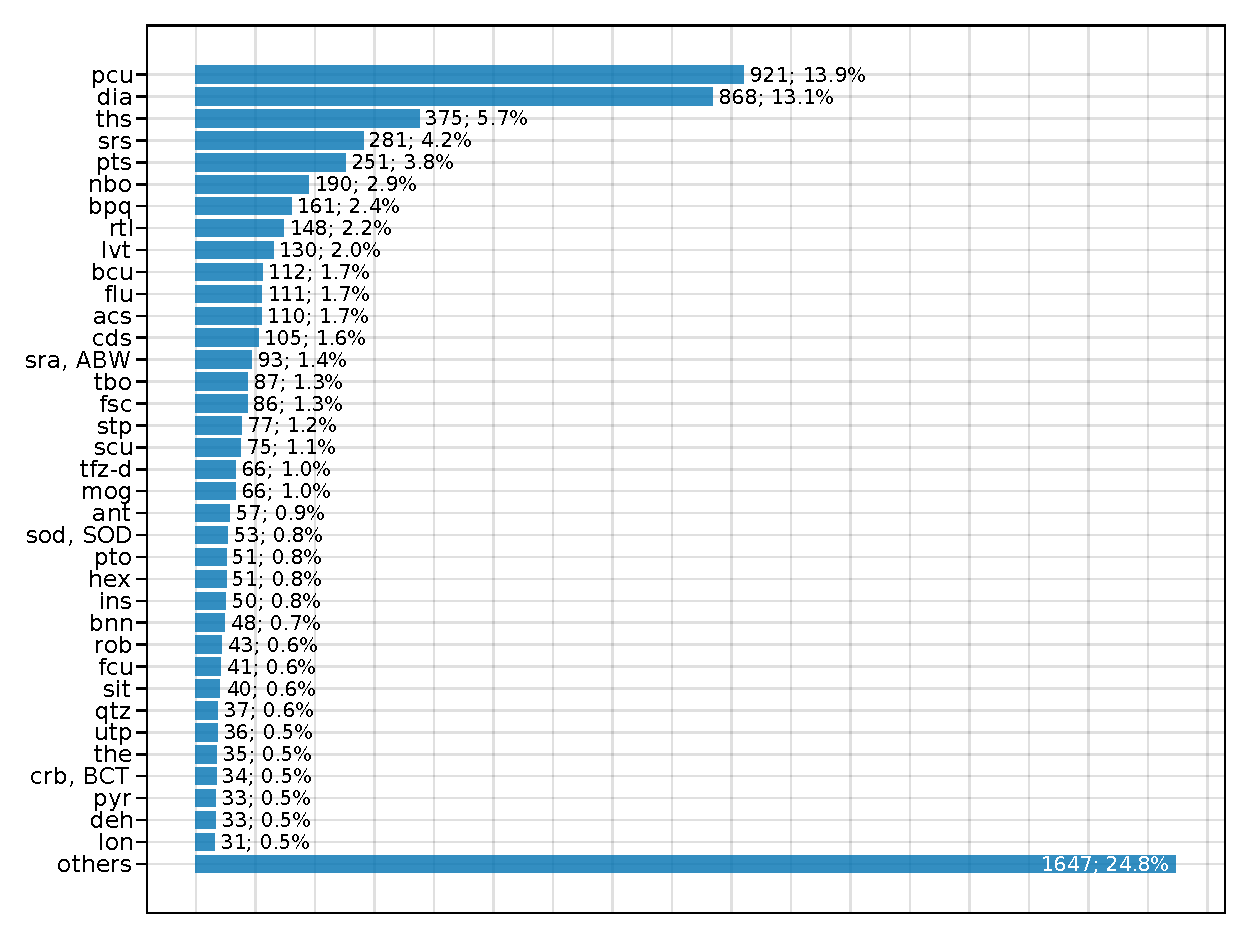
\includegraphics[width=\linewidth]{figures/topology/numstructpernet.pdf}
	\caption{Number of structures per known net in the ordered structures of ASR \autocite{CoREMOF}.}
	\label{numstructpernet}
\end{figure}

Next, let's focus on the 11,190 ordered structures of the ASR subset to avoid duplicates.
The distribution of the number of structures per corresponding net drops faster for unknown nets than for known ones. This is not surprising since known nets should correspond to the most common occurring in nature, whereas unknown nets should only correspond to at most a few corresponding structures. Indeed, among the latter, 1,488 unknown nets only correspond to one MOF structure each, and 302 to two structures. Yet, 5 of them still correspond to thirty MOF structures or more each: I manually checked through the TopCryst interface \autocite{TopCryst} that these 5 nets were part of the ToposPro database, but I could not do so for all the unknown nets since these databases are not open. In comparison, for known nets, 110 of them only correspond to a single MOF structure, 54 to two and 38 to thirty or more each. These most represented nets are detailed in \cref{numstructpernet}: \textbf{pcu} (primitive cubic lattice), \textbf{dia} (diamond) are by far the most common, together accounting for {27\%} of know nets, followed by \textbf{ths}, \textbf{srs} and \textbf{pts}. For zeolitic nets, ABW, SOD (sodalite) and BCT are the most commonly encountered.

The high number of nets with known topologies is a good indicator of the quality of the used clustering algorithm. Yet, since it partly relies on heuristics, it should not be considered fail-proof. To assess its validity, \texttt{CrystalNets.jl} exports both the input and the detected net in VTF format, which can be superposed in a molecular visualisation software to check the correspondence between the vertices of the nets and the expected clusters. I manually checked this correspondence for hundreds of structures with both known and unknown nets, to assert the validity of my implementation. Comparison with TopCryst on many instances seems to indicate that the vast majority of unknown nets encountered in CoRE MOF are not the result of a wrong clustering by \texttt{CrystalNets.jl}, but simply missing from the used databases, probably because they occur on only a handful of actual structures. On the other hand, the proprietary databases of ToposPro appear to include many such nets.

Since this analysis relies solely on \texttt{CrystalNets.jl}, which is independent from the tools used to build and clean the CoRE MOF database, it enabled the identification of 28 improper structures in the database, which were reported.

\subsubsection{Comparison with TopCryst}

I compared \texttt{CrystalNets.jl} and ToposPro, accessed through its online TopCryst interface, on a selection of MOFs common in the literature. The result, presented on \cref{MOFidentification}, shows that both usually return the same topology if it is in the RCSR when using the ``single nodes'' or the `all nodes` clustering options. On the other hand, the ``standard'' clustering leads to different results in several cases. This comes from the difference in clustering heuristics: my implementation regroups each paddle-wheel into a single SBU and removes SBUs made of a lone oxygen (while bonding their neighbors together) while ToposPro does not systematically do so. These two heuristics can be individually toggled off in \texttt{CrystalNets.jl} by the user if necessary. In practice, keeping these heuristics usually leads to less clusters without loss of chemical meaning, which can in turn help identify relevant underlying topologies, like the \textbf{xbi} net for MOF-801 and UiO-66 which contains the information on connectivity between individual metal atoms and with organic linkers. Having access to other clustering options, like ``PE'' also allows considering alternative topological descriptions of the topology.

\newcolumntype{C}[1]{>{\centering\arraybackslash}p{#1}}
\begin{figure}[t]
	\centering
	\begin{tabular}{C{3.1em}C{4.1em}|C{4.8em}C{4.3em}C{4.3em}|C{5.2em}C{6em}|}
		\multicolumn{2}{c|}{\multirow{2}{*}{Name {\scriptsize (CSD identifier)}}} & \multicolumn{3}{c|}{\texttt{CrystalNets.jl}} & \multicolumn{2}{c|}{ToposPro}\\\cline{3-7}
		&& \scriptsize Single/All~Nodes & Standard & PE & \footnotesize Single/All~Nodes & \footnotesize Standard (MOF)\\\hline
		%
		\multicolumn{2}{c|}{HKUST-1 {\scriptsize (LUDLED)}} & \bf tbo & \textbf{tbo} & $\square$ & \bf tbo & 5,6T2 \\\hline
		%
		\multicolumn{2}{c|}{JXUST-1 {\scriptsize (SAXVEW)}} & \bf pcu & $\square$ & $\square$ & \bf pcu & 3,5,5,5T11 \\\hline
		%
		\multicolumn{2}{c|}{MIL-53 {\scriptsize (MINVUA02)}} & \bf bpq/rna & \bf bpq & \textbf{sra}, ABW & $\ast$ & \bf bpq \\\hline
		%\multirow{2}{*}{MIL-53\hspace{-0.5em}} & \scriptsize (POJTOY) & \multirow{2}{*}{{\bf bpq}/{\bf rna}} & \multirow{2}{*}{\bf bpq} & \multirow{2}{*}{\textbf{sra}, ABW} & \multicolumn{2}{c|}{\color{gray}\sl Error: missing symmetries} \\\cline{2-2}\cline{6-7}
		%& \scriptsize (MINVUA02) &&&& $\ast$ & \bf bpq \\\hline
		%
		\multicolumn{2}{c|}{MIL-100 {\scriptsize (BUSPIP)}} & \textbf{moo} & $\square$ & $\square$ & \multicolumn{2}{c|}{\color{gray}\sl Error: timeout} \\\hline
		%
		\multicolumn{2}{c|}{MIL-101 {\scriptsize (OCUNAC)}} & \textbf{mtn-e} & $\square$ & \bf mtn-e-a & \multicolumn{2}{c|}{\color{gray}\sl Error: timeout} \\\hline
		%
		\multicolumn{2}{c|}{MOF-5 {\scriptsize (FIQCEN)}} & \bf tbo & \textbf{tbo} & $\square$ & \bf tbo & 5,6T2 \\\hline
		%
		\multicolumn{2}{c|}{MOF-14 {\scriptsize (QOWRAV)}} & \bf pto & \textbf{pto} & \small sqc11259 & \bf pto & 5,6T46 \\\hline
		%
		\multicolumn{2}{c|}{MOF-177 {\scriptsize (BABRII)}} & $\square$ & $\square$ & $\square$ & 3,3,5,6T36 & \footnotesize 4,4,4,4,4,6,8,8T1 \\\hline
		%
		\multicolumn{2}{c|}{\hspace{-0.4em}MOF-801 {\scriptsize (BOHKAM)}} & \bf fcu & \textbf{xbi} & \bf ubt & \bf fcu & 3,4,8T15 \\\hline
		%
		\multicolumn{2}{c|}{PCN-700 {\scriptsize (RUBLAD)}} & \bf bcu & $\square$ & \textbf{pcb}, ACO & \bf bcu & 3,3,4,6,8T9 \\\hline
		%
		\multicolumn{2}{c|}{UiO-66 {\scriptsize (SURHEU)}} & \bf fcu & \bf xbi & \bf ubt & \bf fcu & 3,4,8T15 \\\hline
		%\multirow{2}{*}{UiO-66} & \scriptsize (RUBTAK) & \multirow{2}{*}{\bf fcu} & \bf \multirow{2}{*}{xbi} & \multirow{2}{*}{\bf ubt} & \multicolumn{2}{c|}{\color{gray}\sl Error: missing symmetries} \\\cline{2-2}\cline{6-7}
		%& \scriptsize (SURHEU) &&&& \bf fcu & 3,4,8T15 \\\hline
		%
		\multicolumn{2}{c|}{ZIF-8 {\scriptsize (FAWCEN)}} & \textbf{sod}, SOD & \textbf{sod}, SOD & \textbf{sod-e} & \textbf{sod}, SOD & \textbf{sod}, SOD \\\hline
		%
		\multicolumn{2}{c|}{ZIF-67 {\scriptsize (GITTOT02)}} & \textbf{sod}, SOD & \textbf{sod}, SOD & \textbf{sod-e} & \textbf{sod}, SOD & \textbf{sod}, SOD \\\hline
		%
	\end{tabular}
	\caption{Comparison of \texttt{CrystalNets.jl} and ToposPro \autocite{ToposPro} (through TopCryst \autocite{TopCryst}) for the identification of topologies on a selection of MOFs.\\
		Topologies in bold come from the RCSR \autocite{RCSR}, in capitals from IZA-SC \autocite{IZA}, sqc11259 comes from EPINET \autocite{EPINET} and the rest are part of ToposPro databases. $\square$ indicates unknown nets.\\
		$\ast$: ToposPro does not provide Single/All Nodes results for MIL-53 but returns \textbf{rna} as ``Standard representation of covalent and ionic compounds'' in addition to \textbf{bpq} as ``Standard representation of coordination compounds and valence-bonded MOFs''.}
	\label{MOFidentification}
\end{figure}

%ToposPro only accepts CIF files containing the explicit list of symmetry operations, while \texttt{CrystalNets.jl} extracts them automatically from the symmetry group name through spglib \autocite{spglib} if they are not provided.
ToposPro may fail for big nets because of the 3-minutes timeout of TopCryst: this happens for MIL-100 and MIL-101 among the tested structures. By comparison, \texttt{CrystalNets.jl} takes less than \SI{10}s to handle them, but these timings are not comparable because the performance of the server on which the TopCryst webservice depends is unknown.

Subsequent to the publication of \cite{CrystalNets}, \textcite{FrankHoffmann} also investigated the difference between TopCryst and the CrystalNets web interface (detailed in \cref{webcrystalnets}). He manually selected \num{100} different MOFs and identified their topology, then compared it with those output by TopCryst and CrystalNets. His results are reproduced in \cref{tab:FrankHoffmann}, where the ``CSD code'' column refers to the name of the structure in the Cambridge Structure Database\autocite{CSD}. On the \num{100} structures, TopCryst correctly identifies \num{68} and CrystalNets \num{80}, which indicates the superiority of the bonding and clustering algorithms used by CrystalNets.

\begin{table}
	\centering
	\footnotesize
	\begin{tabular}{|c|c|l|l|l|}
\hline\textbf{CSD code} & \textbf{Name} & \textbf{Topology} & \textbf{TopCryst} & \textbf{CrystalNets}\\\hline
\bsc{FAVKAP}&\ce{MIL-88}&\textbf{acs}& \cellcolor{green!25}\textbf{acs} & \cellcolor{green!25}\textbf{acs}\\\hline
\bsc{JEJWEB}&\ce{Zn4O(D2-tcppda)_{1.5}}&\textbf{act}& \cellcolor{green!25}\textbf{act} & \cellcolor{red!25}Unknown/\textbf{iac}\\\hline
\bsc{HUHVUD}&\ce{aea-MOF-1}&\textbf{aea}& \cellcolor{red!25}Unknown & \cellcolor{red!25}Unknown\\\hline
\bsc{PIVBEC}&\ce{UMCM-150}&\textbf{agw}& \cellcolor{green!25}\textbf{agw} & \cellcolor{red!25}2-fold \textbf{kgm}\\\hline
\bsc{NEJJIY}&\ce{In-alb-MOF-1}&\textbf{alb}& \cellcolor{red!25}Unknown & \cellcolor{red!25}Unknown\\\hline
\bsc{RAZXIA}&\ce{UTSA-16}&\textbf{ant}& \cellcolor{red!25}Unknown & \cellcolor{red!25}Unknown\\\hline
\bsc{BOHXED}&\ce{MOF-802}&\textbf{bct}& \cellcolor{green!25}\textbf{bct} & \cellcolor{green!25}\textbf{bct}\\\hline
\bsc{FIJDOS}&\ce{MOF-74}&\textbf{bnn}& \cellcolor{red!25}4,8T1 & \cellcolor{red!25}Unknown\\\hline
\bsc{XICYOZ}&\ce{DUT-68}&\textbf{bon}& \cellcolor{red!25}TimeOutError & \cellcolor{red!25}Unknown\\\hline
\bsc{ALECEC}&\ce{NU-1351}&\textbf{cml}& \cellcolor{green!25}\textbf{cml} & \cellcolor{yellow!25}Unknown/\textbf{cml}$^\dagger$\\\hline
\bsc{ICITEU}&\ce{MOF-500}&\textbf{crs}& \cellcolor{green!25}\textbf{crs} & \cellcolor{green!25}\textbf{crs}\\\hline
\bsc{QEFWUV}&\ce{MOF-545}&\textbf{csq}& \cellcolor{green!25}\textbf{csq} & \cellcolor{yellow!25}Unknown/\textbf{csq}\\\hline
\bsc{PEJNOJ}&\ce{MOAAF-1}&\textbf{ctn}& \cellcolor{green!25}\textbf{ctn} & \cellcolor{green!25}\textbf{ctn}\\\hline
\bsc{LIMNUR}&\ce{Zn(dmbd)}&\textbf{dmd}& \cellcolor{green!25}\textbf{dmd} & \cellcolor{green!25}\textbf{dmd}\\\hline
\bsc{RIDCAJ}&\ce{soc-MOF}&\textbf{edq}& \cellcolor{red!25}6,9T9 & \cellcolor{red!25}Unknown\\\hline
\bsc{RUBTAK}&\ce{UiO-66}&\textbf{fcu}& \cellcolor{green!25}\textbf{fcu} & \cellcolor{green!25}\textbf{fcu}\\\hline
\bsc{OLOPUC}&\ce{UTSA-74}&\textbf{fgl}& \cellcolor{yellow!25}Unknown/\textbf{fgl} & \cellcolor{yellow!25}Unknown/\textbf{fgl}\\\hline
\bsc{BEWCUD}&\ce{UNLPF-1}&\textbf{fjh}& \cellcolor{green!25}\textbf{fjh} & \cellcolor{red!25}Unknown/\textbf{scu}\\\hline
\bsc{BOHWIG}&\ce{MOF-841}&\textbf{flu}& \cellcolor{green!25}\textbf{flu} & \cellcolor{green!25}\textbf{flu}\\\hline
\bsc{ANUGEW}&\ce{UMCM-151}&\textbf{fmj}& \cellcolor{green!25}\textbf{fmj} & \cellcolor{green!25}\textbf{fmj}\\\hline
\bsc{JEHBAC}&\ce{[Me2NH2][Mn2(H5L)3)(H2O)2]}&\textbf{fns}& \cellcolor{red!25}3,6T252 & \cellcolor{yellow!25}Unknown/\textbf{fns}\\\hline
\bsc{CESFIQ}&\ce{NOTT-100}&\textbf{fof}& \cellcolor{green!25}\textbf{fof} & \cellcolor{green!25}\textbf{fof}\\\hline
\bsc{RIXPOF}&\ce{MOF-519}&\textbf{fon}& \cellcolor{green!25}\textbf{fon} & \cellcolor{green!25}\textbf{fon}\\\hline
\bsc{HANWAW}&\ce{UTSA-34}&\textbf{frf}& \cellcolor{green!25}\textbf{frf} & \cellcolor{green!25}\textbf{frf}\\\hline
\bsc{JIZLEL}&\ce{PCN-94}&\textbf{ftw}& \cellcolor{green!25}\textbf{ftw} & \cellcolor{yellow!25}Unknown/\textbf{ftw}$^\ddagger$\\\hline
\bsc{VEJZAM}&\ce{ZIF-5}&\textbf{gar}& \cellcolor{green!25}\textbf{gar} & \cellcolor{green!25}\textbf{gar}\\\hline
\bsc{WONJUG}&\ce{gea-MOF-1}&\textbf{gea}& \cellcolor{red!25}Unknown & \cellcolor{green!25}\textbf{gea}\\\hline
\bsc{KOZQEX}&\ce{DUT-75}&\textbf{gee}& \cellcolor{green!25}\textbf{gee} & \cellcolor{green!25}\textbf{gee}\\\hline
\bsc{CAXTUS}&\ce{DUT-42}&\textbf{gra}& \cellcolor{green!25}\textbf{gra} & \cellcolor{green!25}\textbf{gra}\\\hline
\bsc{SOKXOH}&\ce{NU-152}&\textbf{hbk}& \cellcolor{green!25}\textbf{hbk} & \cellcolor{green!25}\textbf{hbk}\\\hline
\bsc{SEMMIJ}&\ce{DUT-126}&\textbf{hbr}& \cellcolor{green!25}\textbf{hbr} & \cellcolor{green!25}\textbf{hbr}\\\hline
\bsc{FIJDEI}&\ce{MOF-72}&\textbf{hex}& \cellcolor{red!25}4,4,5,6T3 & \cellcolor{red!25}Unknown\\\hline
\bsc{ZIJSAO}&\ce{UTSA-61}&\textbf{hey}& \cellcolor{green!25}\textbf{hey} & \cellcolor{green!25}\textbf{hey}\\\hline
\bsc{OFOJEB}&\ce{MOF-893}&\textbf{hfp}& \cellcolor{green!25}\textbf{hfp} & \cellcolor{green!25}\textbf{hfp}\\\hline
\bsc{AZAVUU}&\ce{MOF-890}&\textbf{htp}& \cellcolor{red!25}3,3,4,6T148 & \cellcolor{green!25}\textbf{htp}\\\hline
\bsc{IXETEM}&\ce{pbz-MOF-1}&\textbf{hxg(-b)}& \cellcolor{green!25}\textbf{hxg} & \cellcolor{green!25}\textbf{hxg}\\\hline
\bsc{ACODUT}&\ce{UTSA-30}&\textbf{hyb}& \cellcolor{red!25}\textbf{tsa} & \cellcolor{red!25}\textbf{tsa}\\\hline
\bsc{KEFBII}&\ce{IZE-3}&\textbf{hyx}& \cellcolor{green!25}\textbf{hyx} & \cellcolor{green!25}\textbf{hyx}\\\hline
\bsc{UGEMOK}&\ce{DUT-109}&\textbf{iab}& \cellcolor{red!25}3,4,6T130 & \cellcolor{green!25}\textbf{iab}\\\hline
\bsc{BOHWOM}&\ce{MOF-812}&\textbf{ith}& \cellcolor{green!25}\textbf{ith} & \cellcolor{green!25}\textbf{ith}\\\hline
\bsc{SUKXUS}&\ce{DUT-6}&\textbf{ith-d}& \cellcolor{red!25}4,4,4,6T42 & \cellcolor{red!25}\textbf{pto}\\\hline
\bsc{SUKXUS01}&\ce{MOF-205}&\textbf{ith-d}& \cellcolor{green!25}\textbf{ith-d} & \cellcolor{green!25}\textbf{ith-d}\\\hline
\bsc{OMULAL}&\ce{TPMOF-6}&\textbf{jea}& \cellcolor{red!25}\textbf{hcb} & \cellcolor{red!25}Unknown\\\hline
\bsc{BICPUA}&\ce{UTSA-62}&\textbf{jjt}& \cellcolor{green!25}\textbf{jjt} & \cellcolor{green!25}\textbf{jjt}\\\hline
\bsc{DABQOQ}&\ce{Y-kce-MOF-1}&\textbf{kce}& \cellcolor{red!25}Unknown & \cellcolor{red!25}\textbf{pcu}\\\hline
\bsc{DABQUW}&\ce{Y-kex-MOF-1}&\textbf{kex}& \cellcolor{red!25}Unknown & \cellcolor{red!25}0-dimensional\\\hline
\bsc{AZAVII}&\ce{MOF-888}&\textbf{kgd}& \cellcolor{green!25}\textbf{kgd} & \cellcolor{green!25}\textbf{kgd}\\\hline
\bsc{PACFOP}&\ce{Cu2(py)2(1,3-bdc)2}&\textbf{kgm}& \cellcolor{green!25}\textbf{kgm} & \cellcolor{green!25}\textbf{kgm}\\\hline
	\end{tabular}

	\caption{Comparison of TopCryst and CrystalNets by \textcite{FrankHoffmann}}\label{tab:FrankHoffmann}
	\normalsize
	$^\dagger$: only when using the ``MOF'' structure option. $^\ddagger$: only when using the ``input'' bonding option.
\end{table}

\begin{table}\ContinuedFloat
	\centering
	\footnotesize
	\begin{tabular}{|c|c|l|l|l|}
\bsc{XANLOP}&\ce{UMCM-3}&\textbf{koh}& \cellcolor{green!25}\textbf{koh} & \cellcolor{green!25}\textbf{koh}\\\hline
\bsc{FINMUN}&\ce{NU-1400}&\textbf{lim}& \cellcolor{green!25}\textbf{lim} & \cellcolor{green!25}\textbf{lim}\\\hline
\bsc{GAZCUI}&\ce{DUT-98}&\textbf{llj}& \cellcolor{green!25}\textbf{llj} & \cellcolor{green!25}\textbf{llj}\\\hline
\bsc{CUSJAE}&\ce{FJU-6-TATB}&\textbf{llz}& \cellcolor{red!25}3,9,12T3 & \cellcolor{green!25}\textbf{llz}\\\hline
\bsc{XANKOO}&\ce{CMOF-1}&\textbf{lqm}& \cellcolor{red!25}\textbf{pcu} & \cellcolor{red!25}\textbf{pcu}\\\hline
\bsc{WORREC}&\ce{UTSA-60}&\textbf{lvt}& \cellcolor{green!25}\textbf{lvt} & \cellcolor{green!25}\textbf{lvt}\\\hline
\bsc{FIBKEI}&\ce{PCN-305}&\textbf{mfj}& \cellcolor{green!25}\textbf{mfj} & \cellcolor{green!25}\textbf{mfj}\\\hline
\bsc{NAQKUM}&\ce{USF-3}&\textbf{mmm}& \cellcolor{green!25}\textbf{mmm} & \cellcolor{green!25}\textbf{mmm}\\\hline
\bsc{OCUNAC}&\ce{MIL-101}&\textbf{mtn-e}& \cellcolor{red!25}TimeOutError & \cellcolor{green!25}\textbf{mtn-e}\\\hline
\bsc{YIXBIQ}&\ce{MOF-101}&\textbf{nbo}& \cellcolor{red!25}\textbf{nso} & \cellcolor{green!25}\textbf{nbo}\\\hline
\bsc{MAPMOI}&\ce{[CoCl4]_{0.25}[Co3(\mu^3-OH)(CPT)_{4.5}]}&\textbf{ncb}& \cellcolor{green!25}\textbf{ncb} & \cellcolor{green!25}\textbf{ncb}$^\ddagger$\\\hline
\bsc{MIJRIJ}&\ce{MOF-907}&\textbf{nha}& \cellcolor{green!25}\textbf{nha} & \cellcolor{green!25}\textbf{nha}\\\hline
\bsc{TOVKIA}&\ce{PCN-280}&\textbf{nht}& \cellcolor{red!25}3,3,6T99 & \cellcolor{green!25}\textbf{nht}\\\hline
\bsc{QUSBIP}&\ce{MODF-1}&\textbf{mod}& \cellcolor{green!25}\textbf{mod} & \cellcolor{green!25}\textbf{mod}\\\hline
\bsc{XUDNUH}&\ce{DUT-71}&\textbf{nou}& \cellcolor{green!25}\textbf{nou} & \cellcolor{yellow!25}Unknown/\textbf{nou}\\\hline
\bsc{ALECAY}&\ce{NU-1350}&\textbf{nuc}& \cellcolor{red!25}3,6T22 & \cellcolor{yellow!25}Unknown/\textbf{nuc}$^\dagger$\\\hline
\bsc{MAPHET}&\ce{NU-1301}&\textbf{nun}& \cellcolor{red!25}TimeOutError & \cellcolor{red!25}TimeOutError\\\hline
\bsc{SEMNIJ}&\ce{NU-110}&\textbf{ntt}& \cellcolor{green!25}\textbf{ntt} & \cellcolor{green!25}\textbf{ntt}\\\hline
\bsc{BUYBOO}&\ce{FDM-3}&\textbf{ott}& \cellcolor{red!25}TimeOutError & \cellcolor{green!25}\textbf{ott}\\\hline
\bsc{SAHYOQ}&\ce{MOF-5}&\textbf{pcu}& \cellcolor{green!25}\textbf{pcu} & \cellcolor{green!25}\textbf{pcu}\\\hline
\bsc{HUHWAK}&\ce{pek-MOF-1}&\textbf{pek}& \cellcolor{red!25}Error & \cellcolor{green!25}\textbf{pek}\\\hline
\bsc{TEYZAB}&\ce{MOF-1210}&\textbf{pfm}& \cellcolor{green!25}\textbf{pfm} & \cellcolor{green!25}\textbf{pfm}\\\hline
\bsc{QOWQUO}&\ce{MOF-14}&\textbf{pto}& \cellcolor{green!25}\textbf{pto} & \cellcolor{green!25}\textbf{pto}\\\hline
\bsc{BIMDIL}&\ce{MOF-11}&\textbf{pts}& \cellcolor{green!25}\textbf{pts} & \cellcolor{red!25}Unknown/\textbf{bcu}\\\hline
\bsc{UKOLOV}&\ce{MOF-150}&\textbf{pyr}& \cellcolor{green!25}\textbf{pyr} & \cellcolor{green!25}\textbf{pyr}\\\hline
\bsc{ERIRIG}&\ce{MOF-177}&\textbf{qom}& \cellcolor{green!25}\textbf{qom} & \cellcolor{green!25}\textbf{qom}$^\dagger$\\\hline
\bsc{XICNOO01}&\ce{DUT-67}&\textbf{reo}& \cellcolor{green!25}\textbf{reo} & \cellcolor{green!25}\textbf{reo}\\\hline
\bsc{CUSQEP}&\ce{CTH-6}&\textbf{rtl}& \cellcolor{green!25}\textbf{rtl} & \cellcolor{green!25}\textbf{rtl}\\\hline
\bsc{EPISOM}&\ce{NOTT-140}&\textbf{scu}& \cellcolor{yellow!25}\textbf{mmm}/\textbf{scu} & \cellcolor{yellow!25}\textbf{mmm}/\textbf{scu}\\\hline
\bsc{DOGBEI}&\ce{PCN-224}&\textbf{she}& \cellcolor{red!25}Error & \cellcolor{yellow!25}sqc13549/\textbf{she}\\\hline
\bsc{TUTWUC}&\ce{PCN-223}&\textbf{shp}& \cellcolor{red!25}Error & \cellcolor{yellow!25}Unknown/\textbf{shp}\\\hline
\bsc{LIDDUB}&\ce{PCN-250}&\textbf{edq/soc}& \cellcolor{green!25}\textbf{edq}/\textbf{soc} & \cellcolor{green!25}\textbf{edq}/\textbf{soc}\\\hline
\bsc{RIDCEN}&\ce{In-soc-MOF-1a}&\textbf{edq/soc}& \cellcolor{green!25}\textbf{edq}/\textbf{soc} & \cellcolor{green!25}\textbf{edq}/\textbf{soc}\\\hline
\bsc{UFOROZ}&\ce{Tb-sph-MOF-1}&\textbf{sph}& \cellcolor{red!25}TimeOutError & \cellcolor{yellow!25}Unknown/\textbf{sph}$^\ddagger$\\\hline
\bsc{BOHWUS}&\ce{MOF-808}&\textbf{spn}& \cellcolor{green!25}\textbf{spn} & \cellcolor{green!25}\textbf{spn}$^\ddagger$\\\hline
\bsc{DODBUV}&\ce{PCN-225}&\textbf{sqc}& \cellcolor{yellow!25}sqc7923/\textbf{sqc} & \cellcolor{yellow!25}sqc7923/\textbf{sqc}\\\hline
\bsc{GECXUH}&\ce{MOF-2}&\textbf{sql}& \cellcolor{green!25}\textbf{sql} & \cellcolor{green!25}\textbf{sql}\\\hline
\bsc{KEVWIU}&\ce{(ZnI2)3(tpt)2}&\textbf{srs}& \cellcolor{green!25}\textbf{srs} & \cellcolor{green!25}\textbf{srs}\\\hline
\bsc{LAYRAH}&\ce{ZJNU-74}&\textbf{ssa}& \cellcolor{green!25}\textbf{ssa} & \cellcolor{yellow!25}\textbf{sty}/\textbf{ssa}\\\hline
\bsc{OFOJAX}&\ce{MOF-892}&\textbf{stp}& \cellcolor{green!25}\textbf{stp} & \cellcolor{green!25}\textbf{stp}\\\hline
\bsc{SOKXIB}&\ce{NU-151}&\textbf{sty}& \cellcolor{green!25}\textbf{sty} & \cellcolor{green!25}\textbf{sty}\\\hline
\bsc{DAYMAS}&\ce{Zn(acdc)}&\textbf{sur}& \cellcolor{green!25}\textbf{sur} & \cellcolor{green!25}\textbf{sur}\\\hline
\bsc{FIQCEN}&\ce{HKUST-1}&\textbf{tbo}& \cellcolor{green!25}\textbf{tbo} & \cellcolor{green!25}\textbf{tbo}\\\hline
\bsc{ACOCOM}&\ce{DUT-49}&\textbf{tfb}& \cellcolor{green!25}\textbf{tfb} & \cellcolor{green!25}\textbf{tfb}$^\ddagger$\\\hline
\bsc{EBUCOT}&\ce{[Zn2(btc)]8[Zn2(btc)_{4/3}]3}&\textbf{tfe}& \cellcolor{red!25}\textbf{tbo} & \cellcolor{red!25}\textbf{tbo}\\\hline
\bsc{UNEJEE}&\ce{BUT-12}&\textbf{the}& \cellcolor{green!25}\textbf{the} & \cellcolor{green!25}\textbf{the}\\\hline
\bsc{CUSYAR}&\ce{MOF-210}&\textbf{toz}& \cellcolor{red!25}Error & \cellcolor{green!25}\textbf{toz}\\\hline
\bsc{OVOKOB}&\ce{MOF-910}&\textbf{tto}& \cellcolor{red!25}3,4,11T2 & \cellcolor{red!25}Unknown\\\hline
\bsc{ZECRAC}&\ce{DUT-25}&\textbf{ttz}& \cellcolor{green!25}\textbf{ttz} & \cellcolor{green!25}\textbf{ttz}\\\hline
\bsc{TAKKIC}&\ce{UHM-25}&\textbf{ucp}& \cellcolor{green!25}\textbf{ucp} & \cellcolor{green!25}\textbf{ucp}\\\hline
\bsc{TIZQOK}&\ce{DUT-32}&\textbf{umt}& \cellcolor{green!25}\textbf{umt} & \cellcolor{green!25}\textbf{umt}\\\hline
\bsc{HOGLEV}&\ce{PCN-12}&\textbf{zhc}& \cellcolor{green!25}\textbf{zhc} & \cellcolor{green!25}\textbf{zhc}\\\hline
	\end{tabular}

	\caption{Comparison of TopCryst and CrystalNets by \textcite{FrankHoffmann} (continued)}
	\normalsize
	$^\dagger$: only when using the ``MOF'' structure option. $^\ddagger$: only when using the ``input'' bonding option.
\end{table}

\subsection{Database of aluminophosphates}

Additionally, I surveyed the topologies of Zheng, Li and Yu's database of aluminophosphates \autocite{ALPO}. These 385 experimental structures are given as CIF files with little to no cleaning from the publications they stem from. In particular, solvent is included and the structures can contain multiple overlapping atoms with partial occupancy, while atoms of the main structure are often partially substituted. \texttt{CrystalNets.jl} automatically removes 0-dimensional residues like solvent and keeps for each site only the atom with the highest occupancy. %Using the default heuristics for both bonding and clustering of vertices, w\texttt{CrystalNets.jl} recognise {56\%} of the 210 3D nets in the database. This number rises to {65\%} when using the ``zeolite'' structure option, which enforce 2-connectivity for oxygens and otherwise uses the same bonding rules as MOFs, and up to
Using the ``Zeolite'' structure option of \texttt{CrystalNets.jl}, the software recognises {64\%} of the 205 3D nets in the database. This number rises to {73\%} by adding a heuristic to remove P--O--P and Al--O--Al linkages, which are usually not accounted for when computing the topologies of AlPOs.

\begin{figure}[t]
	\centering
	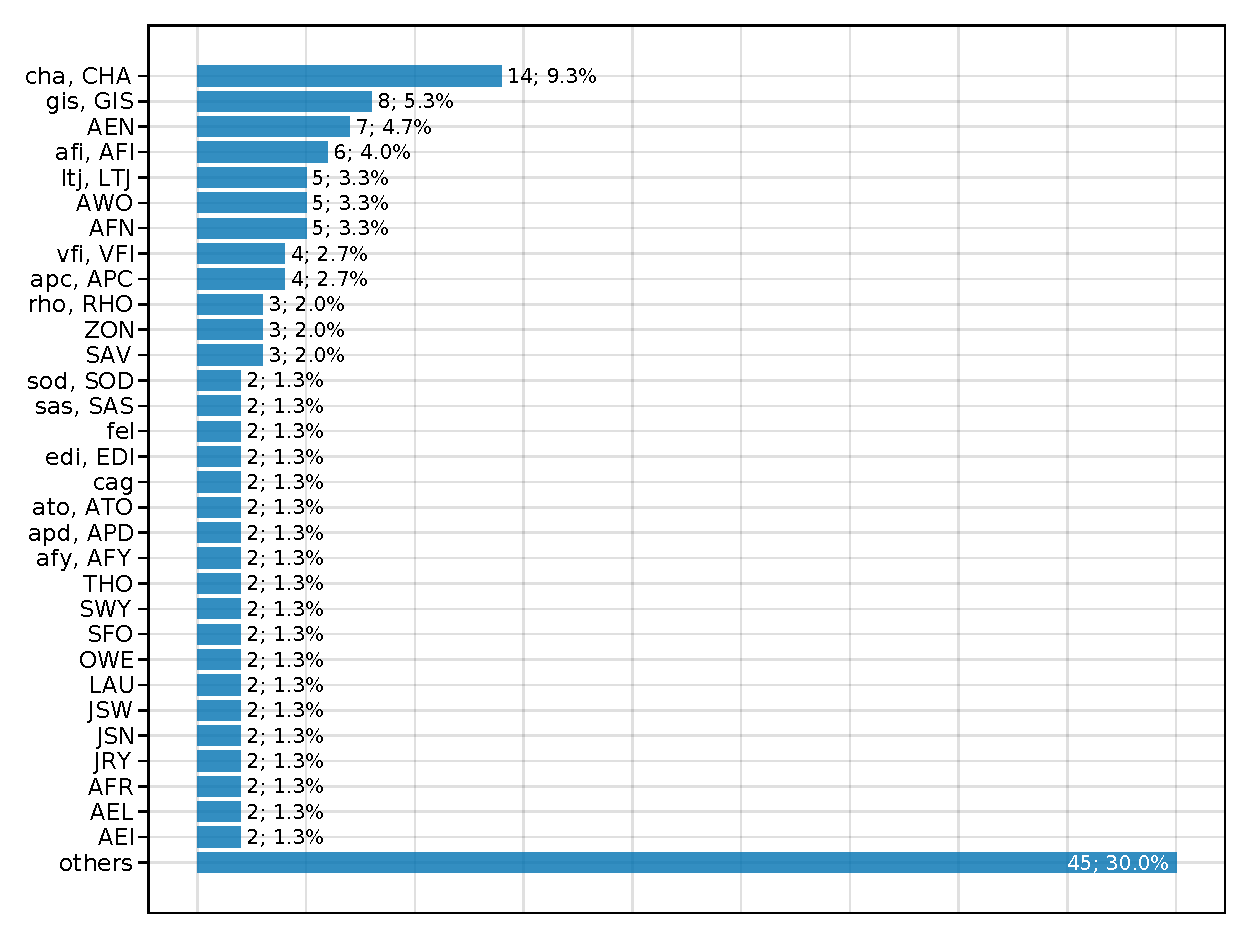
\includegraphics[width=\linewidth]{figures/topology/numstructpernetalpos.pdf}
	\caption{Number of structures per known net in the ALPO database \autocite{ALPO}.}
	\label{numstructpernetalpos}
\end{figure}

The 31 known nets represented on more than one structure in the database are represented on \cref{numstructpernetalpos}. With the exception of \textbf{fel} (originating from feldspars) and \textbf{cag} (occuring in variscite), they are all referenced in the database of zeolite frameworks of IZA-SC. This is expected since AlPOs are structurally close to zeolites, with the replacement of Si atoms by Al and P. Conversely, it shows that \textbf{fel} and \textbf{cag} may be nets underlying the structure of unreported zeolites, especially since both only have 4-coordinates vertices, corresponding to the T-atoms, and can be embedded to exhibit pores.

Most known structures have a net represented only once (45 nets \textit{i.e.} {30\%}) or twice (19 nets \textit{i.e.} {25\%}). In comparison, among the unknown nets, 1 occurs on three structures, 5 on two and the 32 others appear only once each. Both distribution tails and comparison of known and unknown nets follow a pattern similar to the CoRE MOF database.\\

For the structures for which the underlying net has been recognised as one of the IZA-SC, there is little doubt on the validity of the detected net. For the others however, there is no systematic way of determining whether the detected net is indeed that representing the structure or not except from visually checking the adequate superposition of the detected net and the initial framework for each file. This limitation comes from the lack of cleaning of the input CIF files, which can lead \texttt{CrystalNets.jl} to interpret solvent residues as part of the framework for instance, or duplicate atoms as two different atoms instead of one. This issue can be circumvented by either cleaning the CIF inputs, as in the CoRE MOF database, or by manually checking the correspondence if working on individual files. Obviously, this limitation is inherent to the quality of the input files and affects all topology determination codes.

\subsection{Hypothetical zeolites}

% For zeolites only, also cite Kriber, EUTAX, TOPOLAN, ZeoTsites and TOTOPOL (see TOTOPOL paper 10.1016/j.micromeso.2005.08.024)

The study of framework topology has historically been extensively applied to zeolites \autocite{TopochemistryZeolites}. One reason is that the structure of zeolites, made only from tetrahedral (T = Si, Al, \ldots) atoms bridged by T--O--T linkages, is simple enough to show an almost one-to-one correspondence between each framework and its underlying net. Using this fact, large databases of hypothetical zeolites have been devised: the core idea consists in embedding 4-connected nets in real space, either by enumeration of the nets \autocite{Treacy} or by Monte Carlo sampling of vertex positions \autocite{Deem}. The vertices correspond to Si atoms while O atoms are placed along the edges. Each obtained structure is subsequently refined by minimizing its energy through molecular dynamics and with simulated annealing.

Since these structures are built from their underlying net, I tried to perform the opposite operation on the Predicted Crystallography Open Database (PCOD) \autocite{Deem} to assess my implementation. This database contains 331,172 CIF files representing zeolites with energies within \SI{30}{kJ/mol} (per SiO$_2$ unit) of $\alpha$-quartz, which were analyzed by \texttt{CrystalNets.jl} in 45 minutes using 20 cores (Intel Xeon Silver 4210R CPUs, 2.4~GHz). Bond guessing forced O atoms to have at most 2 neighbours, which is the default heuristic for O atoms not bound to metals: this incidentally ensures that all vertices of the net correspond to Si atoms.

As the \ce{SiO4} tetrahedra are somewhat distorted during the refinement steps, the bonds guessed from the resulting structure do not always correspond to those from which it was built. As a result, there were 11 frameworks whose T-atoms were not all 4-connected, and 75 other frameworks whose coordination sequences did not match that recorded in the database. Two structures were found to have the same underlying net: 8013876 and 8035701, the latter having different detected coordination sequences than indicated.
Barring these 86 mismatched structures, 18 nets only have a 2D periodicity and 31 are unstable nets not handled by \texttt{CrystalNets.jl}. All those ``problematic'' nets represent less than 0.04\% of all nets in the database. For the rest, no two structures had the same underlying net.

Indeed, by construction of the database, structures whose topology is already part of the database are removed. The invariants used to identify the topology are the coordination sequences and the ring sizes: this strategy does ensure that no two structures with the same net are present, but it is too restrictive since two distinct nets could share these invariants. In the future, the use of a unique topological identifier through \texttt{CrystalNets.jl} could thus potentially lead to the generation of more structures.

\section{Web interface}
\label{webcrystalnets}
%\subsection{General presentation}

\begin{figure}
	\centering
	\begin{subfigure}{\linewidth}
		\centering
		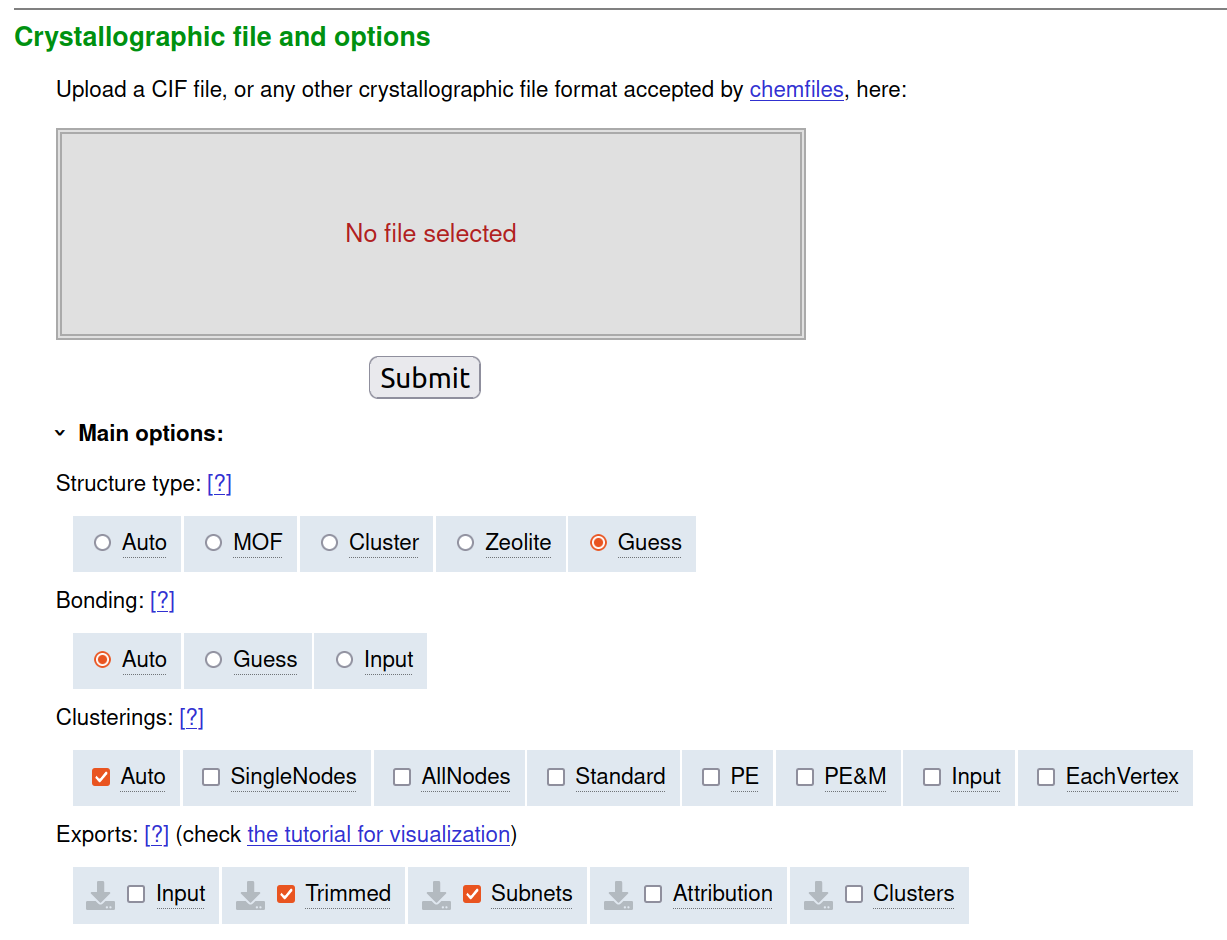
\includegraphics[width=0.9\linewidth]{figures/topology/WebsitePrompt.png}
		\subcaption{Input prompt with the main options including the structure, bonding and clustering algorithms, and visualization outputs. More advanced options exist below.}
	\end{subfigure}

\vfill

	\begin{subfigure}{\linewidth}
		\centering
		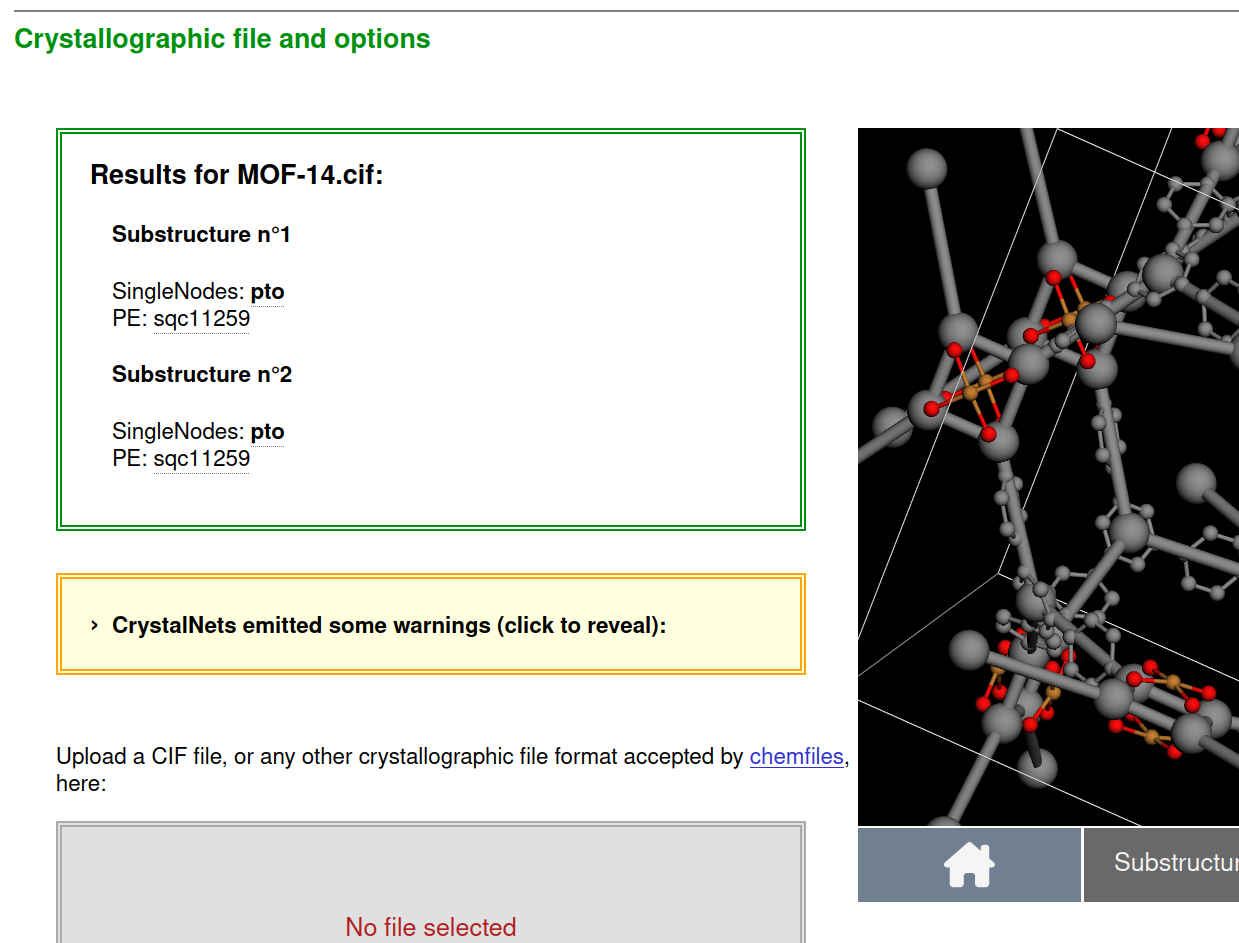
\includegraphics[width=0.9\linewidth]{figures/topology/WebsiteAnswer.png}
		\subcaption{Response page, including the results and a visualization panel on the right (truncated here)}
	\end{subfigure}
	\caption{CrystalNets web interface}\label{fig:crystalnetsweb}
\end{figure}

CrystalNets is the web interface to the \texttt{CrystalNets.jl} Julia library, accessible online at \url{https://progs.coudert.name/topology}. The focus of this online tool is to provide easier handling than its programmatic back-end, to make it maximally accessible. Its interface, presented on \cref{fig:crystalnetsweb} simply consists in an input box where the user can drag-and-drop or browse the input file. The main options are visible below, with pre-selected default values. These main options include the type of material, which may guide the automatic choice of the subsequent options, the bonding algorithm (whether automatic as discussed above, or using the input), the clustering strategy, and some visualization export choices.
A panel of advanced options, folded by default, can also be accessed to tweak the cutoff radii of the bonding algorithm or toggle the aromatic cycle detection, among other choices.

Once the input and options have been selected, typing Enter or clicking the ``Submit'' sends the request to a server, which internally calls the \texttt{CrystalNets.jl} library with the correct input, formats the answer and transfers it to the user. The resulting page contains a green box with the identified topologies, as well as a visualization panel on the right.
Visualization files can be downloaded by clicking on the icon next to the required  exports: they are in VTF or PDB format, which can be used by VMD.
A yellow box, folded by default, may also appear in case \texttt{CrystalNets.jl} emitted some warnings or information statements.
If an error occurred, or if no net can be extracted (as may happen with a non-periodic input), a red box detailing the error appears.
In any case, the HTML result page contains all the information; it can thus be saved locally and reopened at a later time if need be.\\

%Let's now discuss the visualization panel and the internals of our webserver implementation.

%\subsection{Topology visualization}

The visualization panel on the right of the result page relies on the 3Dmol.js library. This choice was mainly driven by its reactivity when displaying even large crystals, as well as its ease of manipulation. As with any such visualization tool, dragging the canvas rotates the crystal while zooming in or out is done with the mousewheel. The home button on the left resets the viewer position and zoom. Clicking on the right-most button, or double-clicking the canvas, displays it across the entire webpage, which can be convenient to focus on visualization.

The middle buttons control what is currently being displayed. Each button either directly controls a visible element, \textit{e.g.} the button showing the input crystal or its trimmed version, or it reveals a menu with other buttons. For instance, each substructure of an interpenetrated crystal has its own menu. Navigating these menus thus allows interactively choosing the visible elements on the canvas, to enable, for example, focusing on the superposition of the input crystal and the ``All Nodes'' representation of its second substructure only.\\

%\subsection{Implementation}

The server handling the requests is written with the Bottle library in Python. Upon receiving a user query for CrystalNets, it calls a custom code written in Julia, passing on the input and related options.

This code relies on the \texttt{DaemonMode.jl} library to minimize the experienced latency. Indeed, Julia works with a Just-In-Time (JIT) compilation paradigm, which enables highly specialized compilation of code leading to very fast execution. The counterpart of this strategy is the compilation time incurred each time a function is called with a new set of argument types. Several mitigation strategies have been implemented in Julia, to reduce this ``time to first execution'', the three main ones being writing type-ground code to reduce the amount of total compilation, hunting invalidation to prevent code from being re-compiled after loading and using precompilation to effectively compile part of the code ahead of time. The practical gains due to these strategies is considerable, especially with the advent of native code caching as part of precompilation in Julia v1.9.

However, the latency requirements of a webserver are particularly stringent, since this waiting time is immediately felt by the user. \texttt{DaemonMode.jl} is a Julia library offering an alternative latency-reduction scheme, well adapted to this use-case. Instead of launching a new Julia process with each request, it captures each query and forwards it to a single Julia process that operates all of them. JIT compilation can then be performed on the unique process at startup, and any subsequent Julia call will simply be executed by the same process, without the need to compile anything at all, effectively resulting in an ahead-of-time compilation of the necessary codebase.

Depending on the load state of the server, it appears that most requests can be served within a few seconds at most, the only cases exceeding ten seconds being very large nets for which the latency time is negligible with respect to the actual processing time of the net identification algorithm.

\section{Summary and perspectives}

\texttt{CrystalNets.jl} is a Julia library that implements topology identification on crystalline materials. The core algorithm for topology detection is strongly inspired from that used in Systre \autocite{Systre} which computes a topological genome, that is a sequence of numbers uniquely identifying the net underlying the given structure. The algorithmic and implementation improvements of \texttt{CrystalNets.jl} still preserve the soundness and polynomial time complexity of the initial algorithm, while offering a much better performance across all kinds of nets: it is on average 56 times faster than Systre and up to thousands of times faster in some cases. Moreover, the software directly takes crystallographic files as input and can automatically detect bonds if they are absent; it also includes a general clustering algorithm with different target options for framework materials, and heuristics adapted to metal--organic frameworks specifically.

Overall, \texttt{CrystalNets.jl} was successfully tested against a large diversity of crystalline structures: MOFs, aluminophosphates, zeolites and many other crystals. Even on large databases, the program shows great performance and can reliably recognise any structure in the Systre archive of the RCSR, in the IZA-SC database of zeolite structures and in EPINET. It successfully attributes known topologies to {60\%} of the structures in CoRE MOF after automatically clustering the vertices according to the ``single nodes'' policy. It was also able to recognise {73\%} aluminophosphate structures from Zheng \textit{et al.}'s database \autocite{ALPO}, automatically removing solvent residues and colliding atoms when possible.

\texttt{CrystalNets.jl} can be used as a faster and more convenient alternative to Systre and ToposPro for the identification of nets underlying crystalline structures. Its programmatic interface can be integrated to any computational pipeline written in Julia, as well as some other languages through bindings. %Looking forward, we plan on providing a website interface similar to TopCryst \autocite{TopCryst}, which could be useful to compare any structure to one of those surveyed in the previously exposed databases. %We also plan on including results from the topological survey of the COD \autocite{COD} and CSD \autocite{CSD} databases. The latter could then serve as comparison for our bonding and clustering algorithms against those of ToposPro \autocite{BlatovCSD}.

\end{document}